%Version 3 December 2023
% See section 11 of the User Manual for version history
%
%%%%%%%%%%%%%%%%%%%%%%%%%%%%%%%%%%%%%%%%%%%%%%%%%%%%%%%%%%%%%%%%%%%%%%
%%                                                                 %%
%% Please do not use \input{...} to include other tex files.       %%
%% Submit your LaTeX manuscript as one .tex document.              %%
%%                                                                 %%
%% All additional figures and files should be attached             %%
%% separately and not embedded in the \TeX\ document itself.       %%
%%                                                                 %%
%%%%%%%%%%%%%%%%%%%%%%%%%%%%%%%%%%%%%%%%%%%%%%%%%%%%%%%%%%%%%%%%%%%%%

%%\documentclass[referee,sn-basic]{sn-jnl}% referee option is meant for double line spacing

%%=======================================================%%
%% to print line numbers in the margin use lineno option %%
%%=======================================================%%

%%\documentclass[lineno,sn-basic]{sn-jnl}% Basic Springer Nature Reference Style/Chemistry Reference Style

%%======================================================%%
%% to compile with pdflatex/xelatex use pdflatex option %%
%%======================================================%%

%%\documentclass[pdflatex,sn-basic]{sn-jnl}% Basic Springer Nature Reference Style/Chemistry Reference Style


%%Note: the following reference styles support Namedate and Numbered referencing. By default the style follows the most common style. To switch between the options you can add or remove “Numbered” in the optional parenthesis. 
%%The option is available for: sn-basic.bst, sn-vancouver.bst, sn-chicago.bst%  
 
%%\documentclass[pdflatex,sn-nature]{sn-jnl}% Style for submissions to Nature Portfolio journals
%%\documentclass[pdflatex,sn-basic]{sn-jnl}% Basic Springer Nature Reference Style/Chemistry Reference Style
\documentclass[pdflatex,sn-mathphys-num]{sn-jnl}% Math and Physical Sciences Numbered Reference Style 
%%\documentclass[pdflatex,sn-mathphys-ay]{sn-jnl}% Math and Physical Sciences Author Year Reference Style
%%\documentclass[pdflatex,sn-aps]{sn-jnl}% American Physical Society (APS) Reference Style
%%\documentclass[pdflatex,sn-vancouver,Numbered]{sn-jnl}% Vancouver Reference Style
%%\documentclass[pdflatex,sn-apa]{sn-jnl}% APA Reference Style 
%%\documentclass[pdflatex,sn-chicago]{sn-jnl}% Chicago-based Humanities Reference Style

%%%% Standard Packages
%%<additional latex packages if required can be included here>

\usepackage{graphicx}%
\usepackage{multirow}%
\usepackage{amsmath,amssymb,amsfonts}%
\usepackage{amsthm}%
\usepackage{mathrsfs}%
\usepackage[title]{appendix}%
\usepackage{xcolor}%
\usepackage{textcomp}%
\usepackage{manyfoot}%
\usepackage{booktabs}%
\usepackage{algorithm}%
\usepackage{algorithmicx}%
\usepackage{algpseudocode}%
\usepackage{listings}%
\usepackage{makecell}
\newcommand{\tabitem}{\makebox[1em][r]{\textbullet}\hspace{0.5em}}
%%%%

%%%%%=============================================================================%%%%
%%%%  Remarks: This template is provided to aid authors with the preparation
%%%%  of original research articles intended for submission to journals published 
%%%%  by Springer Nature. The guidance has been prepared in partnership with 
%%%%  production teams to conform to Springer Nature technical requirements. 
%%%%  Editorial and presentation requirements differ among journal portfolios and 
%%%%  research disciplines. You may find sections in this template are irrelevant 
%%%%  to your work and are empowered to omit any such section if allowed by the 
%%%%  journal you intend to submit to. The submission guidelines and policies 
%%%%  of the journal take precedence. A detailed User Manual is available in the 
%%%%  template package for technical guidance.
%%%%%=============================================================================%%%%

%% as per the requirement new theorem styles can be included as shown below
\theoremstyle{thmstyleone}%
\newtheorem{theorem}{Theorem}%  meant for continuous numbers
%%\newtheorem{theorem}{Theorem}[section]% meant for sectionwise numbers
%% optional argument [theorem] produces theorem numbering sequence instead of independent numbers for Proposition
\newtheorem{proposition}[theorem]{Proposition}% 
%%\newtheorem{proposition}{Proposition}% to get separate numbers for theorem and proposition etc.

\theoremstyle{thmstyletwo}%
\newtheorem{example}{Example}%
\newtheorem{remark}{Remark}%

\theoremstyle{thmstylethree}%
\newtheorem{definition}{Definition}%

\raggedbottom
%%\unnumbered% uncomment this for unnumbered level heads

\begin{document}

\title[Article Title]{Article Title}

%%=============================================================%%
%% GivenName	-> \fnm{Joergen W.}
%% Particle	-> \spfx{van der} -> surname prefix
%% FamilyName	-> \sur{Ploeg}
%% Suffix	-> \sfx{IV}
%% \author*[1,2]{\fnm{Joergen W.} \spfx{van der} \sur{Ploeg} 
%%  \sfx{IV}}\email{iauthor@gmail.com}
%%=============================================================%%

\author*[1,2]{\fnm{First} \sur{Author}}\email{iauthor@gmail.com}

\author[2,3]{\fnm{Second} \sur{Author}}\email{iiauthor@gmail.com}
\equalcont{These authors contributed equally to this work.}

\author[1,2]{\fnm{Third} \sur{Author}}\email{iiiauthor@gmail.com}
\equalcont{These authors contributed equally to this work.}

\affil*[1]{\orgdiv{Department}, \orgname{Organization}, \orgaddress{\street{Street}, \city{City}, \postcode{100190}, \state{State}, \country{Country}}}

\affil[2]{\orgdiv{Department}, \orgname{Organization}, \orgaddress{\street{Street}, \city{City}, \postcode{10587}, \state{State}, \country{Country}}}

\affil[3]{\orgdiv{Department}, \orgname{Organization}, \orgaddress{\street{Street}, \city{City}, \postcode{610101}, \state{State}, \country{Country}}}

%%==================================%%
%% Sample for unstructured abstract %%
%%==================================%%

\abstract{Federated learning is a distributed machine learning paradigm that emerged as a solution to the need for privacy
protection in artificial intelligence. Like traditional machine
learning, federated learning is threatened by multiple attacks,
such as backdoor attacks,
Byzantine attacks, and adversarial attacks. The weaknesses are
exacerbated by the inaccessibility of data in federated learning,
which makes it more difficult to defend against these threats.
This points to the need for further research into defensive
approaches to make federated learning a real solution for distributed machine learning paradigm with securing data privacy.
Our survey provides a taxonomy of these threats and defense
methods, describing the general situation of this vulnerability
in federated learning. We also sort out
the relationship between these methods, their advantages and
disadvantages, and discuss future research
directions regarding the security issues of federated learning
from multiple perspectives.}

%%================================%%
%% Sample for structured abstract %%
%%================================%%

% \abstract{\textbf{Purpose:} The abstract serves both as a general introduction to the topic and as a brief, non-technical summary of the main results and their implications. The abstract must not include subheadings (unless expressly permitted in the journal's Instructions to Authors), equations or citations. As a guide the abstract should not exceed 200 words. Most journals do not set a hard limit however authors are advised to check the author instructions for the journal they are submitting to.
% 
% \textbf{Methods:} The abstract serves both as a general introduction to the topic and as a brief, non-technical summary of the main results and their implications. The abstract must not include subheadings (unless expressly permitted in the journal's Instructions to Authors), equations or citations. As a guide the abstract should not exceed 200 words. Most journals do not set a hard limit however authors are advised to check the author instructions for the journal they are submitting to.
% 
% \textbf{Results:} The abstract serves both as a general introduction to the topic and as a brief, non-technical summary of the main results and their implications. The abstract must not include subheadings (unless expressly permitted in the journal's Instructions to Authors), equations or citations. As a guide the abstract should not exceed 200 words. Most journals do not set a hard limit however authors are advised to check the author instructions for the journal they are submitting to.
% 
% \textbf{Conclusion:} The abstract serves both as a general introduction to the topic and as a brief, non-technical summary of the main results and their implications. The abstract must not include subheadings (unless expressly permitted in the journal's Instructions to Authors), equations or citations. As a guide the abstract should not exceed 200 words. Most journals do not set a hard limit however authors are advised to check the author instructions for the journal they are submitting to.}

\keywords{Federated Learning \sep Trustworthy Artificial Intelligence \sep Non-IID data \sep Robust Model }

%%\pacs[JEL Classification]{D8, H51}

%%\pacs[MSC Classification]{35A01, 65L10, 65L12, 65L20, 65L70}

\maketitle

\section{Introduction}
Artificial intelligence (AI) can analyze large amounts
of data and solve complex problems in various fields.
Most existing state-of-the-art AI techniques rely on
rich and high-quality datasets to train a highly accurate
machine learning model. For example, while training
the SAM model, Alexander et al.~\cite{kirillov2023segment} build the largest
segmented dataset ever, building more than 1 billion
masks on 11 million images. However, in more practical reality,
most companies cannot construct such large and highquality datasets as Meta when training their model. To
address this problem, one possible solution is the sharing
of data among multiple organizations or companies to
collaboratively train models.

But collaborative training presents several new challenges while it has developed rapidly.
The first challenge stems from data privacy. The data held
by organizations may contain sensitive information, such
as medical or financial data of their users. Additionally,
new legal frameworks are increasingly emphasizing the
protection of individual data privacy~\cite{voigt2017eu}. Privacy protection introduces restrictions that prevent privacy data from
leaving its originating organization and being uploaded
to central server. The second challenge is related to the
diverse organizations of data. Data from different organizations provides an increase in available data, driving
advancements in artificial intelligence models. However,
due to the various organizations, storing and processing
data from different organizations, as well as reducing communication costs between these organizations have
become a new challenge.
\begin{figure}[t]
	\centering

	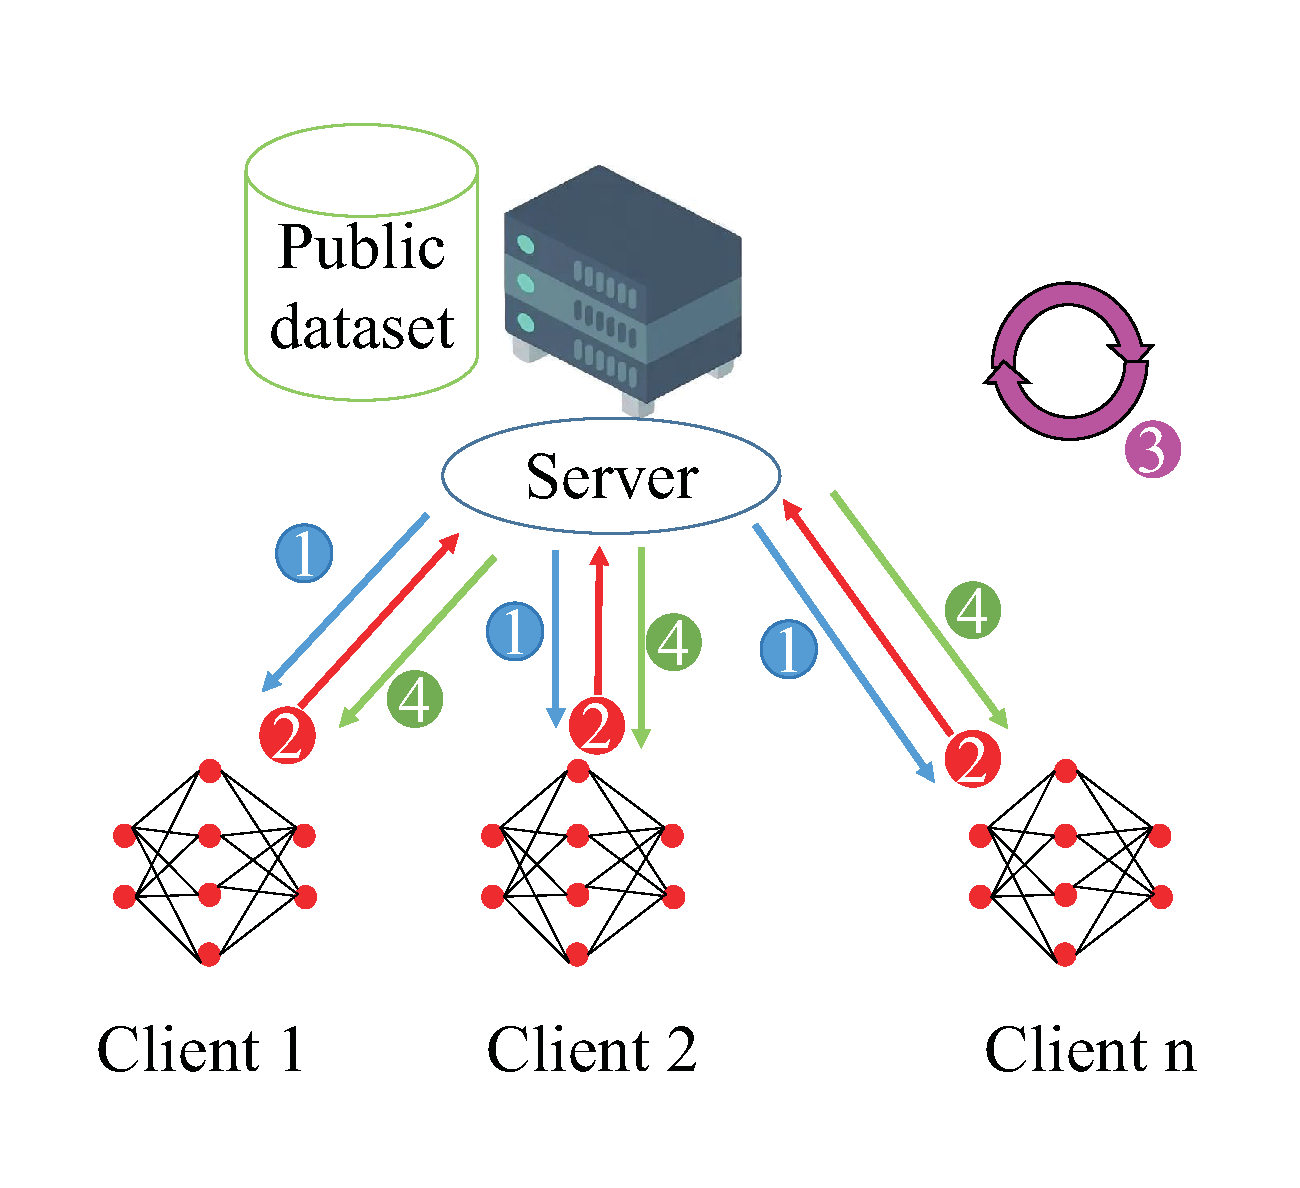
\includegraphics[width=1.0\linewidth,height=3.5in]{output/fig1.eps}
	\caption{A schematic of federated learning.
		Each iteration of federated learning can be divided into four steps.
		1: The central server sending the initialized global model to the client. 2: The
		clients then train locally and submit the local updates to the server. 3: The server performs the model aggregation.
		4: the server sends the aggregated model to the clients.}
	\label{fig1}
\end{figure}  

In response to such challenges, Google~\cite{mcmahan2017communication} develops a
distributed machine learning framework called federated
learning (FL). This framework allows each client to collectively train models without sharing their data. The data
of each client remains private and inaccessible to others
during training process. As shown in Fig.~\ref{fig1}, in a typical federated learning framework, the server firstly sends a global
model to all selected clients as local models. These clients
then use their local datasets to train the local models and
upload their trained model updates to the central server.
After receiving the updates from all selected clients, the
server updates the global model by averaging the uploaded
updates. And the server sends the updated global model
to the selected clients. Completing the four steps, one iteration
of federated learning is complete. The entire federated
learning requires multiple iterations to make model achieve
convergence. Throughout the training process, only the
data owners have access to their local data. This approach
ensures the protection of data from unauthorized access
by other clients or the central server, while also reducing
communication costs between the clients and the server~\cite{yang2019federated}. Due to the advantages of FL, FL has been widely
applied to many fields in recent years~\cite{doshi2022federated,becking2022adaptive,liu2024vertical,liu2024recent,ye2024openfedllm,gecer2024federated}.
However,
further research has shown that federated learning also
faces numerous security risks~\cite{yazdinejad2024robust,zhang2024a3fl,rodriguez2023survey,tariq2023trustworthy,zhang2023survey} like backdoor
attacks, adversarial attacks, and Byzantine attacks.  
\begin{figure}[t]
	\centering
	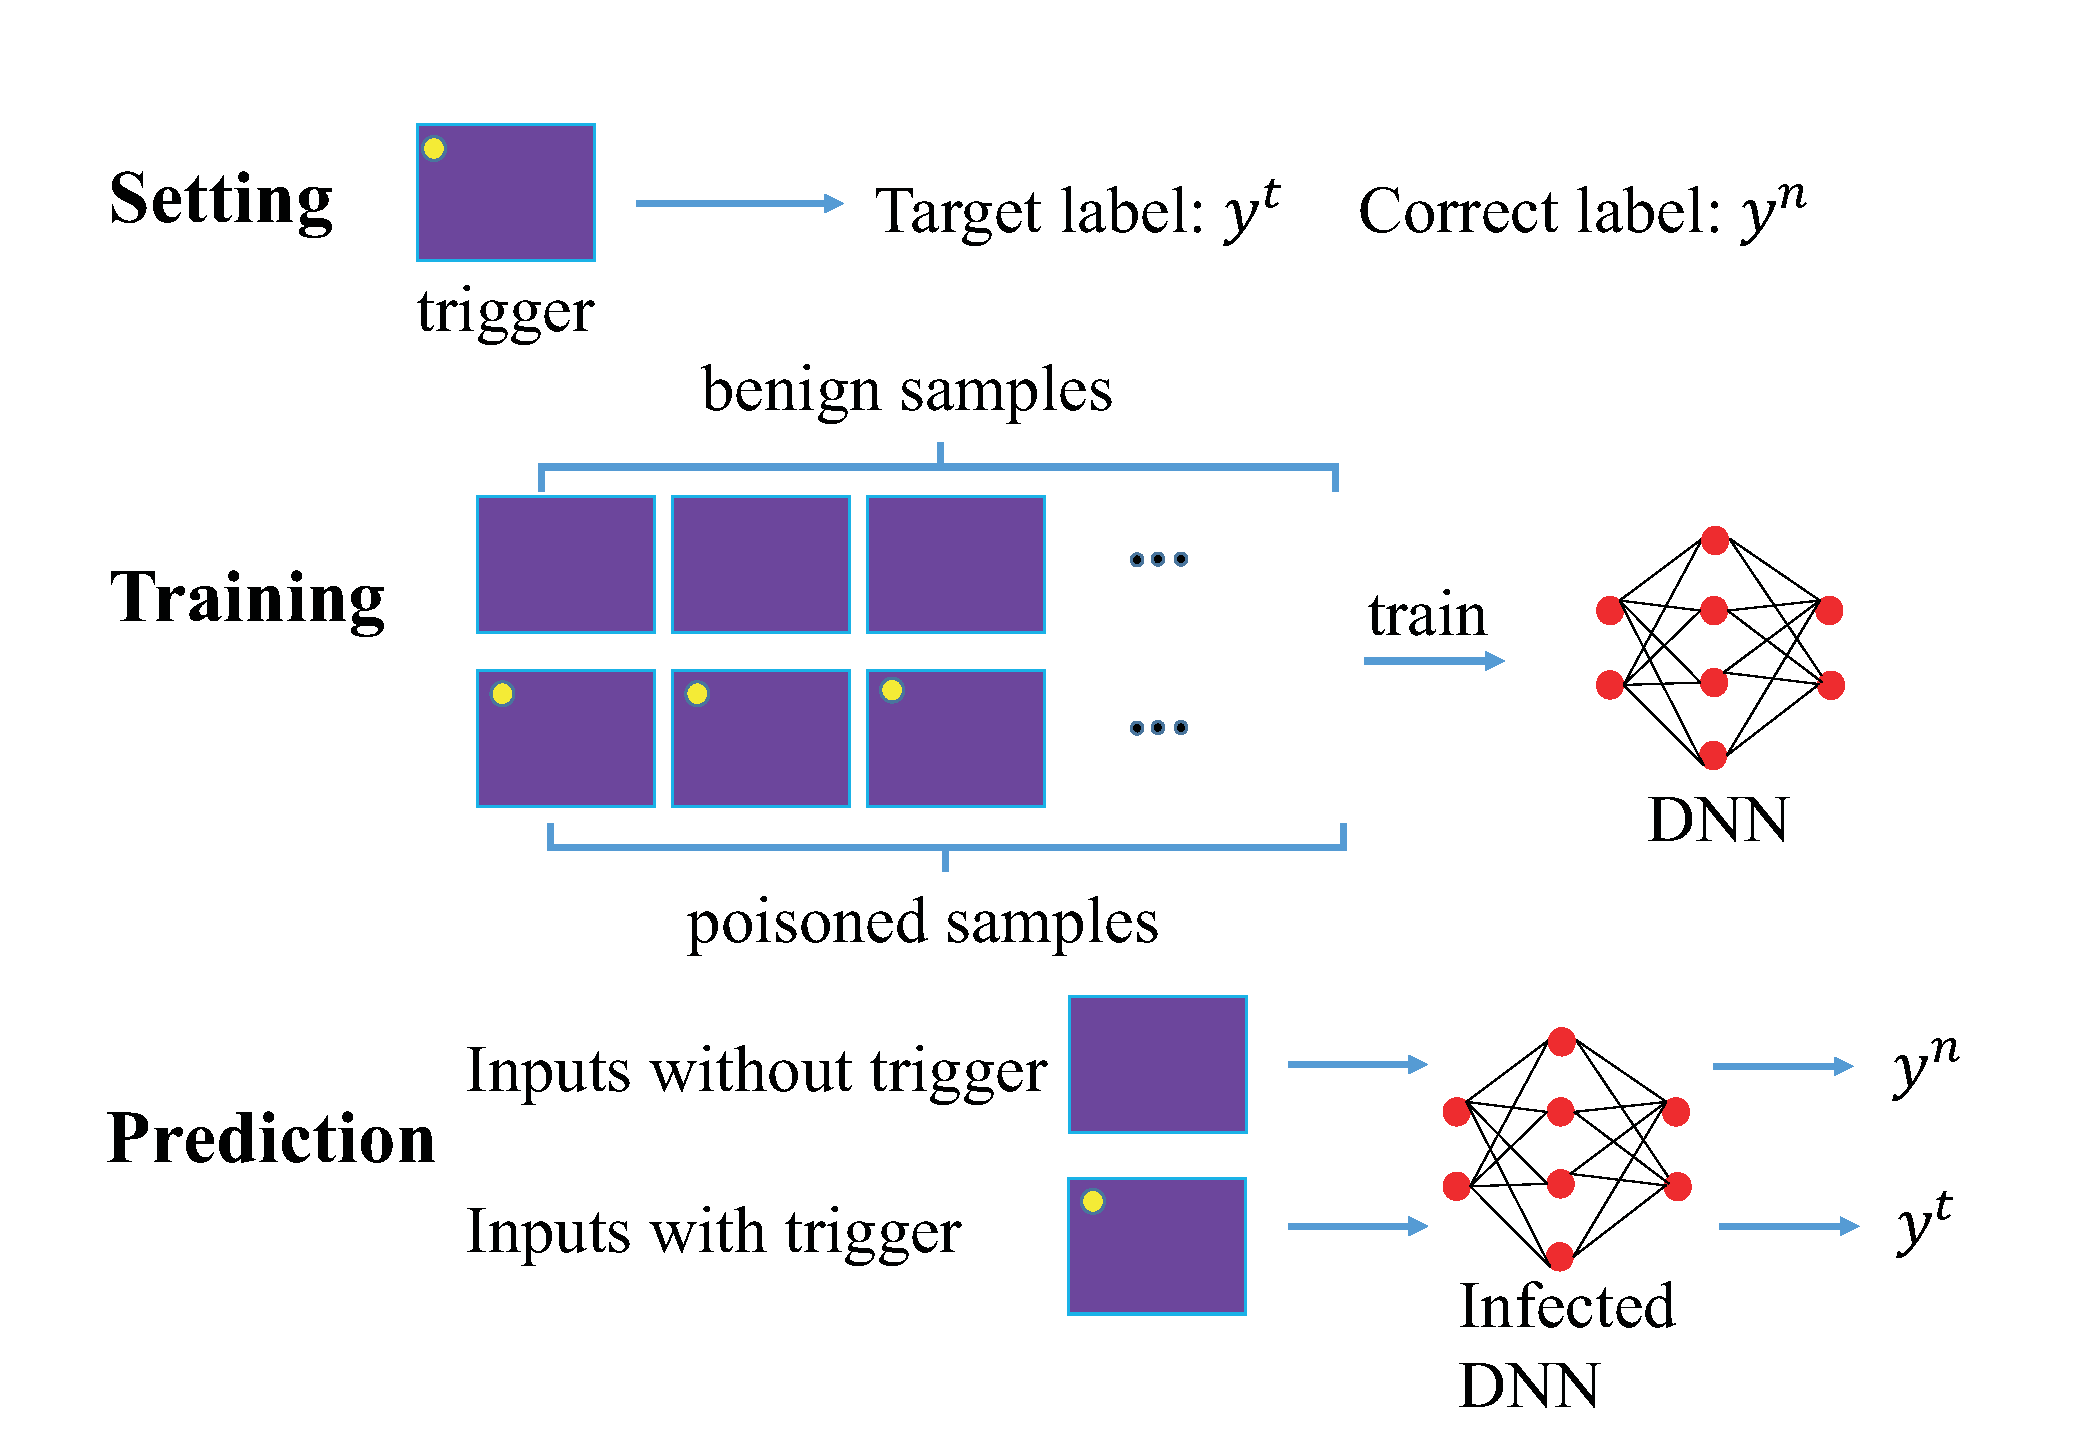
\includegraphics[width=1.0\linewidth,height=3in]{output/fig2.eps}
	\caption{As shown in the figure, a common backdoor attack method
		is to insert backdoor samples during model training, so that the
		model can show the predicted results desired by the attacker on the
		backdoor samples during prediction.}
	\label{fig2}
\end{figure}

\begin{figure}[t]
	\centering
	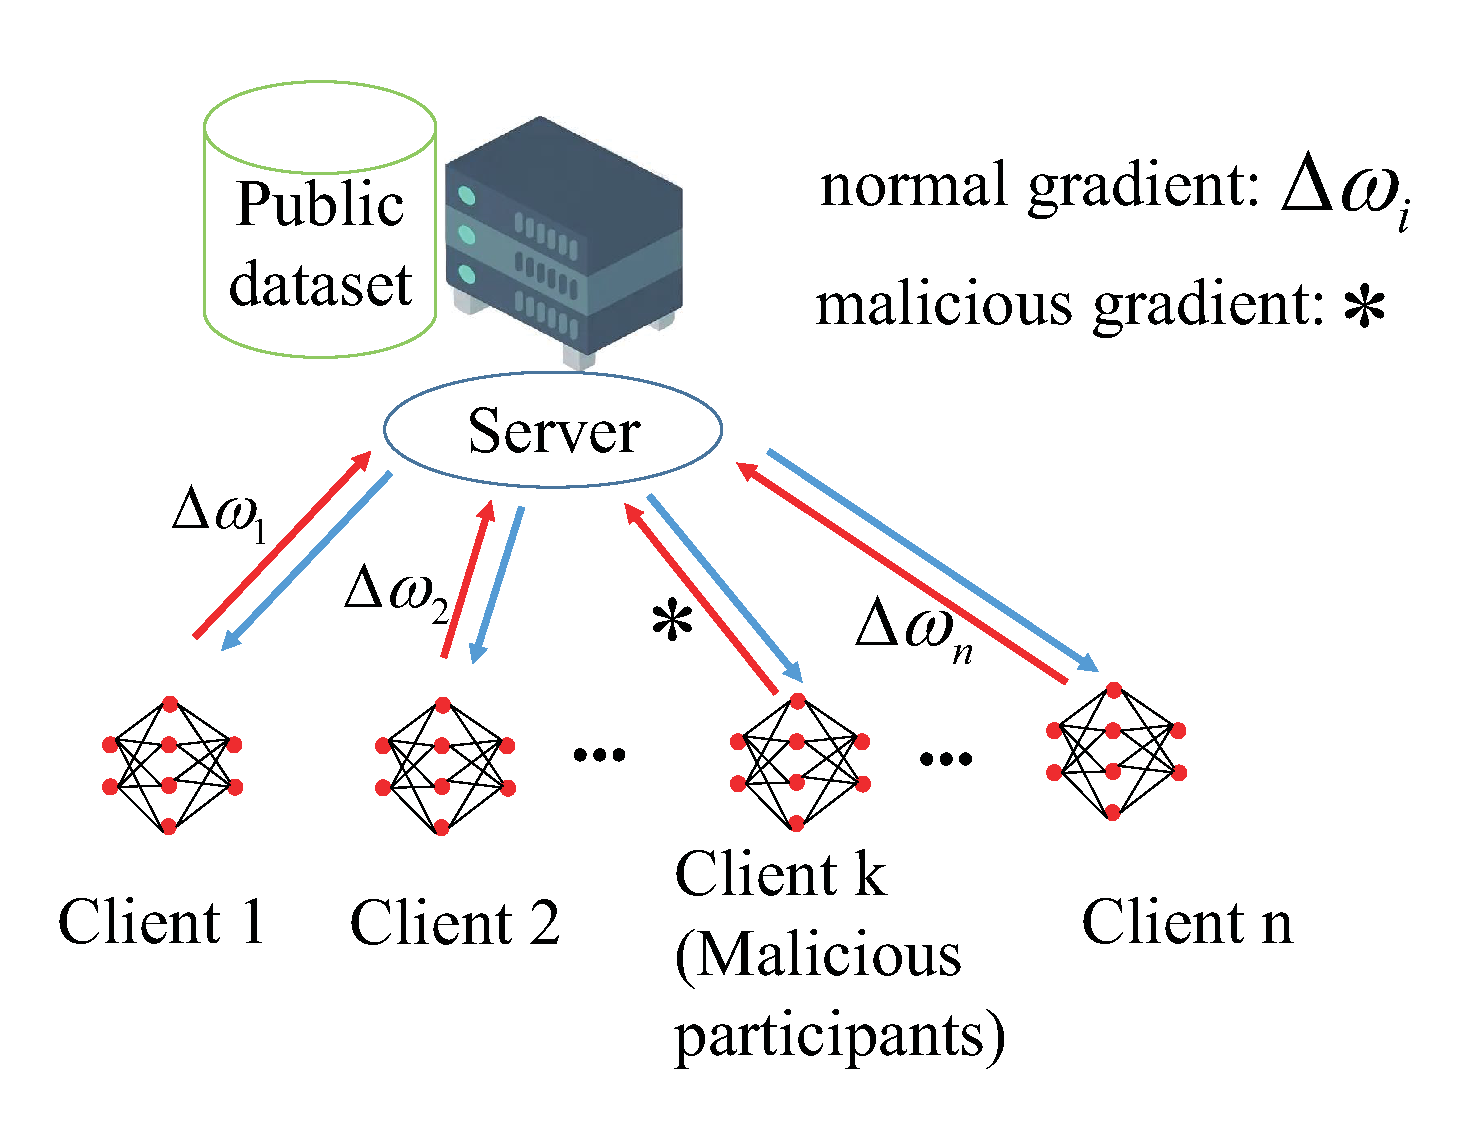
\includegraphics[width=1.0\linewidth,height=3in]{output/fig3.eps}
	\caption{In Byzantine attacks, there exist one or more malicious
		participants(client k) in the federated learning system who disrupt
		the training process by sending incorrect or misleading updates to
		the central server, causing abnormal convergence.}
	\label{fig3}
\end{figure}  

\begin{table*}[t]
	\caption{\textbf{Comparison of Attacks}}
	\label{Comparison of Attacks}
	\scriptsize
	\centering
	\resizebox{\textwidth}{!}{ 
	\begin{tabular}{|c|c|c|c|c|} % 有七列,使用 "c" 表示居中对齐,没有竖线
		\toprule % 第一道横线
		\textbf{Attack Category} & \textbf{Goal}                                        & \textbf{Mechanism} & \textbf{Attack Phase} & \textbf{Targeted Attack} \\
		\midrule
		Backdoor Attack          & \makecell[tl]{\tabitem Present results as attackers                                                                          \\ expect on the backdoor samples. \\ \tabitem Behave normally  on benign samples.} & \makecell[tl]{Excessive learning ability of models.} & Training & Targeted \\
		\midrule
		Byzantine Attack         & \makecell[tl]{\tabitem Reduce model generalization.                                                                          \\ \tabitem Make model difficult to converge.} & \makecell[tl]{Distribution of federated learning clients.} & Training & Untargeted\\
		\midrule
		Adversarial Attack       & \makecell[tl]{\tabitem Misclassify attacked samples.                                                                         \\ \tabitem Behave normally on benign samples.} & \makecell[tl]{The difference of samples in feature space.} & Inference & Targeted / Untargeted \\
		\toprule
		% 继续插入更多数据行
	\end{tabular}
	}
\end{table*}


We primarily enumerate backdoor attacks, adversarial
attacks, and Byzantine attacks in federated learning, along
with their corresponding defense methods~\cite{pan2024one,yang2024distributed,zeng2021rethinking,wang2024rope,doan2020februus,li2020learning, naseri2024badvfl}. These attacks
pose significant threats to federated learning systems,
and in response to these new threats, several FL defense
methods have been proposed. In previous surveys~\cite{nguyen2024backdoor,zhang2024survey,rodriguez2023survey,tariq2023trustworthy,zhang2023survey}, researchers have explored some attacks and defense
strategies in the context of federated learning.
We do not believe that this classification between the two types of attacks can be perfect
cause some attack methods~\cite{bagdasaryan2020backdoor, zhang2022neurotoxin, zhou2021deep, sun2022semi} start from the aspect of modifying the client model.
These surveys often categorize backdoor attacks and Byzantine
attacks as data poisoning attacks and rarely delve into
adversarial attacks in the field of federated learning. In
this survey, we propose a new classification approach for
these two types of attacks and provide an overview of their
corresponding defense mechanisms. We also supplement this paper with content on adversarial attacks
and their defense mechanisms. Furthermore, we conduct
a detailed analysis of the effectiveness and limitations
of these attack methods and their corresponding defense
mechanisms. In section \ref{Threat Models}, we give a preliminary introduction to the
definitions of the three attacks discussed in this survey and try to find their commonalities.
In section \ref{Backdoor Attack}-\ref{Defenses against Adversarial Attack}, we introduce the current state of attack and defense methods for each of the three threats.
Finally, we analysis the advanced research and problems faced by federated learning in section \ref{Advanced Research and Problems}.

\section{Threat Models}
\label{Threat Models}
In this section, we give a preliminary introduction to the
definitions of the three attacks discussed in this survey.


\textbf{Backdoor attacks}~\cite{bagdasaryan2020backdoor,wang2020attack,gong2022backdoor,sun2019can,ozdayi2021defending} refer to a
malicious backdoor added to the global model by malicious
participants during training process. The backdoor can be
triggered by specific inputs, allowing attackers to control
the outputs of the model. The goal of backdoor attack is to make the model maintain correct outputs on benign samples,
while presenting the bad results as attackers expect on backdoor samples as shown in Fig.~\ref{fig2}, .

\begin{figure}[h]
	\centering
	\includegraphics[width=1.0\linewidth,height=2.8in]{output/fig4.eps}
	\caption{Adversarial attacks require adding subtle and carefully
		crafted perturbations to the input data to deceive the model and
		cause it to make incorrect predictions.}
	\label{fig4}
\end{figure}

\textbf{Byzantine attacks}~\cite{fang2020local,guo2021byzantine,prakash2020mitigating} is that there exist one
or more malicious participants in the federated learning
system who disrupt the training process by sending
incorrect or misleading updates to the central server, causing
abnormal convergence, as shown in Fig.\ref{fig3}. 



\textbf{Adversarial attacks}~\cite{zizzo2020fat,chen2022calfat,li2023federated,zhang2023delving}
require adding subtle and carefully crafted perturbations
to the input data to deceive the model and cause it to
make incorrect predictions as shown in Fig.\ref{fig4}.

These attacks have different goals, mechanisms, and
attack stages. We can categorize these threats into two main stages: the training phase and
the inference phase. Additionally, we can also categorize
them between untargeted attacks and targeted attacks
based on whether a specific target is present or not. And
we make a comparison among attacks in Tab.~\ref{Comparison of Attacks}.

\subsection{Attack in Training Phase \& Attack in Inference Phase}
(1)Attack in Training Phase: Attacks during the model
training process are intended to impact
the federated learning model. During the training
stage, backdoor attacks involve the insertion of a backdoor
into the model, whereas input deception models with
triggers are utilized during the reasoning stage to cause
the model to generate incorrect results~\cite{miao2018towards,zhang2019data}. Byzantine
attacks disrupt the convergence of the model by utilizing
malicious clients or servers~\cite{fang2020local}. It causes the global model fail to converge by sending harmful information or disrupt communication.

(2)Attack in Inference Phase: Attacks that occur during the
reasoning phase are typically intended to alter the model's
reasoning outcomes and deceive it into generating incorrect
outputs~\cite{barreno2006can} . Adversarial attacks leverage the model's
vulnerability to disturbances and utilize samples with
adversarial perturbations as input to the model, causing
it to produce erroneous outcomes.

\subsection{Untargeted Attack \& Targeted Attack}
(1)Untargeted attacks: Untargeted attacks are designed
to compromise the integrity of the target model in
arbitrary manner. Byzantine attack is one form of untargeted
attacks that involves uploading malicious gradients to the
server in an arbitrary manner, with the goal of causing
the global model to fail~\cite{lamport2019byzantine,xie2020fall,bernstein2018signsgd,damaskinos2019aggregathor}.

(2)Targeted Attacks: A targeted attack is executed with
the aim of inducing the model to produce the target label
specified by the adversary for specific testing examples,
while keeping the testing error for other testing examples
unaffected~\cite{damaskinos2019aggregathor}. Backdoor attack is a typical application
of targeted attacks. 


\section{Backdoor Attack}
\label{Backdoor Attack}

\begin{table*}[t]
	\caption{\textbf{Comparison of Backdoor Attacks}}
	\label{Comparison of Backdoor Attacks}
	\centering
	\resizebox{\textwidth}{!}{ 
	\begin{tabular}{|c|c|c|c|c|} % 有七列,使用 "c" 表示居中对齐,没有竖线
		\toprule % 第一道横线
		\textbf{Attack Method}       & \textbf{Category}          & \textbf{Persistence}                           & \textbf{Mechanism}                      & \textbf{Stealthiness}                          \\
		\midrule
		\makecell{Semantic Backdoor} & \makecell{Model Poisoning} & \makecell{$\star$}                             & \makecell{Model replacement.}           & \makecell{$\star$}                             \\
		\midrule
		\makecell{Label Flipping}    & \makecell{Data Poisoning}  & \makecell{$\star$}                             & \makecell{Generated poisoned examples.} & \makecell{$\star$}                             \\
		\midrule
		\makecell{CLean Label}       & \makecell{Data Poisoning}  & \makecell{$\star$$\star$$\star$ }              & \makecell{Sample camouflage.}           & \makecell{$\star$$\star$$\star$$\star$$\star$} \\
		\midrule
		\makecell{Transferable                                                                                                                                                                                \\ Clean Label} & \makecell{Data Poisoning} & \makecell{$\star$$\star$$\star$$\star$} & \makecell{Sample camouflage.} & \makecell{$\star$$\star$$\star$$\star$} \\
		\midrule
		\makecell{Backdoor with                                                                                                                                                                               \\ Edge Data} & \makecell{Data Poisoning} & \makecell{$\star$$\star$} & \makecell{Long-tail distribution.} & \makecell{$\star$$\star$$\star$} \\
		\midrule
		\makecell{Distributed                                                                                                                                                                                 \\ Backdoor} & \makecell{Data Poisoning} & \makecell{$\star$} & \makecell{Embedded backdoors distributed \\ from multiple clients.} & \makecell{$\star$$\star$$\star$$\star$} \\
		\midrule
		\makecell{Neurotoxin}        & \makecell{Model Poisoning} & \makecell{$\star$$\star$$\star$$\star$$\star$} & \makecell{Attack parameters that                                                         \\ change less during training.} & \makecell{$\star$$\star$$\star$} \\
		\midrule
		\makecell{Optimization-based                                                                                                                                                                          \\Backdoor Attack} & \makecell{Model Poisoning} & \makecell{$\star$$\star$$\star$} & \makecell{Optimization method} & \makecell{$\star$$\star$}  \\
		\midrule
		\makecell{Distance Awareness                                                                                                                                                                          \\Attack} & \makecell{Model Poisoning} & \makecell{$\star$$\star$$\star$} & \makecell{Attacking Distance-aware Attack} & \makecell{$\star$$\star$$\star$} \\
		\midrule
		\makecell{Dynamic Backdoor                                                                                                                                                                            \\Attack} & \makecell{Data Poisoning} & \makecell{$\star$$\star$} & \makecell{Dynamic backdoor} & \makecell{$\star$$\star$$\star$$\star$$\star$} \\
		\midrule
		\makecell{Chameleon}         & \makecell{Data Poisoning}  & \makecell{$\star$$\star$$\star$$\star$}        & \makecell{Adaptive technique.}          & \makecell{$\star$$\star$$\star$}               \\

		\toprule
		% 继续插入更多数据行
	\end{tabular}}
\end{table*}

Backdoor attacks on deep neural networks require
malicious backdoors to be secretly implanted in the model.
This enables the model to function normally when
processing benign inputs, but triggers pre-defined malicious
behavior when presented with a specific malicious trigger.
The first neural backdoor in centralized settings can be
traced back to 2013~\cite{geigel2013neural,gu2017badnets}.
Due to the unique nature of federated learning,
whereby the model is trained on individual clients, it is
more susceptible to backdoor attacks compared to the
general centralized training model. These backdoor attacks
in federated learning can be divided into two categories
based on the different stages at which the adversary
inserts backdoors into the training pipeline: data poisoning
attacks and model poisoning attacks.

\subsection{Data Poisoning Attack}
In data poisoning attacks, it is assumed that the
adversary has full control over the training data collection
process of compromised clients. Then the poisoned dataset
typically consists of a combination of clean data with
ground-truth labels and data with backdoor triggers that
have targeted labels.

(1)Visible Poisoning: Early methods~\cite{bagdasaryan2020backdoor,gong2022backdoor} of backdoor
attacks in federated learning can rely on a single trigger,
meaning that all corrupted clients inject the same trigger
with their local training datasets. The triggers are usually predetermined, such as a
square located at redundant pixels in the image. During
reasoning, the inserted triggers are used on malicious
clients to activate the aggregation model~\cite{bagdasaryan2020backdoor,gong2022backdoor}. While
the effectiveness of inserting the backdoor has been shown
to be significant, the aforementioned approach merely
transfers backdoor attacks from centralized learning
directly to federated learning, without fully leveraging the
distributed nature of the latter. This is because the same
triggers are embedded in all adversarial clients. Some
studies ~\cite{xie2019dba} take advantages of federated learning to carry out
backdoor attacks. As shown in Fig.~\ref{fig5}, Xie et al.~\cite{xie2019dba} propose
a distributed backdoor attack (DBA) that decomposes a
global trigger pattern, similar to a centralized attack, into
local patterns and embeds them into different malicious
clients. Compared to traditional methods that insert the
same trigger, DBA is more efficient and covert due to
its hidden local trigger mode, making it easier to bypass
robust aggregation rules.

\begin{figure}[h]
	\centering
	\includegraphics[width=1.0\linewidth,height=3.5in]{output/fig5.eps}
	\caption{DBA decomposes a global trigger pattern, similar to a
		trigger in centralized attack, into local patterns and embeds them
		into different malicious clients.}
	\label{fig5}
\end{figure}

But distributed backdoors are also easy to detect
because the triggers are static. And if the static triggers are
changed to dynamic, the backdoors will be more difficult
to detect. Salem et al.~\cite{salem2022dynamic} conduct a clear and systematic
study on the feasibility of dynamic flip-flops, which can
facilitate the backdoor attacks by generating antagonistic
network algorithms to create triggers. This way, the same
tags can be hijacked with different trigger patterns that
share similar potential representations and positions. Li
et al.~\cite{li2020rethinking} also conduct a direct investigation of dynamic
triggers. These triggers can be flexibly produced during the
attack phase, as they maintain their effectiveness even
under substantial changes. The results of the study show
that dynamically triggered backdoor attacks are more
powerful, and they require new techniques to be defeated
because they break the static trigger hypothesis of most
current defense systems. Despite the potential threats of data poisoning attacks
in federated learning, they face many practical limitations
due to the unique distributed characteristics~\cite{wang2020attack}. This
is because the data distribution and model aggregation
steps in federated learning tend to neutralize most of
the contributions of the backdoor model, leading to rapid
forgetting of the backdoor by the global model. In light of
this situation, Wang et al.~\cite{wang2020attack} propose selecting poisoning
samples from edge data to reduce the forgetting effection
caused by model updating.

Dai et al.~\cite{dai2023chameleon} propose a new backdoor attack method
called Chameleon, which enables attackers to create more
persistent visual backdoors by adapting to peer-to-peer
images. The durability of the backdoor largely depends on
the existence of two types of identical benign images that
are closely related to the toxic image: Interferers, which
are images that share the same original tag as the toxic
image. And facilitators, which are images with the target
back tag. Interferers can cause update conflicts between
toxic updates and benign updates, which may reduce the
accuracy of the backdoor. Conversely, facilitators can help
reintroduce backdoor information into the federated
learning model and mitigate the catastrophic forgetting effect
after the attacker leaves the training process. Inspired by
these observations, Chameleon is designed to amplify these
effects and enhance the durability of the backdoor.

(2)Invisible Poisoning: In this context, the term
'invisible' denotes the user's ability to execute a backdoor attack
on a sample without requiring any additional actions to
be performed on the sample itself. Label flipping is a widely recognized attack in
centralized machine learning (ML), as demonstrated in previous
research studies~\cite{shen2016auror,steinhardt2017certified}. In addition, it is also a suitable
method for the federated learning (FL) scenario, given its
adversarial goal and capabilities~\cite{tolpegin2020data}. As shown in Fig.~\ref{fig6},
some of the samples labeled 'dog' are flipped to 'cat' and
the samples of 'cat' are flipped to 'dog'.

\begin{figure}[h]
	\centering
	\includegraphics[width=1.0\linewidth,height=2.2in]{output/fig6.eps}
	\caption{Label Flipping.In this picture, some of the samples labeled
		'dog' are flipped to 'cat' and the samples of 'cat' are flipped to 'dog'.}
	\label{fig6}
\end{figure}

Nevertheless, the label flipping technique has its
limitations since it necessitates modifying the label of the
samples, making it less practical. Thus, an attack technique
that is more covert and can deceive manual inspection
would be more appealing in this scenario. As shown in
Fig.~\ref{fig7}, clean-label attack preserves the label of the poisoned
data, and the manipulated image still appears to be a
benign sample~\cite{shafahi2018poison,zhu2019transferable}. This type of attack leverages feature
collision, where the crafted poison examples continue to
resemble the source instances in visual appearance, while
being closer to the targeted instances in the latent feature
space. Data poisoning faces the risks of being easily detected
and traced. At the same time, the initial assumption that
the attacker has complete control over the data set is
difficult to achieve in many scenarios.

\subsection{Model Poisoning Attack}
To address the limitations of data poisoning attacks,
we can not only focus on improving the data poisoning
technology itself, but also exploring the potential of model
poisoning techniques. Since the average method is the
most widely used approach for aggregating local updates
from clients, a simple way to amplify the backdoor effect
is to prioritize updates from adversarial clients over those
from benign clients.

\begin{figure}[h]
	\centering
	\includegraphics[width=1.0\linewidth,height=2.5in]{output/fig7.eps}
	\caption{Clean-label attack preserves the label of the poisoned data,
		and the manipulated image still appears to be a benign sample. As
		you see, it’s almost impossible to tell the difference between poisoned
		examples and benign examples.}
	\label{fig7}
\end{figure}

Bagdasaryan et al.~\cite{bagdasaryan2020backdoor} propose the first backdoor
attack against federated learning. Their approach involves
training a backdoor model that closely resembles the
global model, which is then used to replace the latest
global model. To improve the effectiveness of this
replacement, they slow down the learning rate to extend
the lifespan of the backdoor model, and add an anomaly
detection term to the loss function to avoid detection.
This strategy requires careful evaluation of the global
parameters and performs better when the global model
is close to convergence.

But similar to data poisoning, such direct substitutions
are easily detected. In order to avoid such substitutions,
Zhou et al.~\cite{zhang2022neurotoxin} propose an optimization-based model
poisoning attack that involves injecting adversarial
neurons into the redundant space of a neural network to
maintain the attack's concealment and persistence. To
identify the redundant space, the Hessian matrix is used
to measure the updated distance and direction of each
neuron's main task. An additional term is then added
to the loss function to prevent poisoned neurons from
being injected in locations that are particularly relevant
to the main task. In a similar vein, Zhang et al.~\cite{zhou2021deep}
propose a persistent backdoor attack called Neurotoxin.
This method relies on the empirical observation that the
norm of a stochastic gradient is primarily concentrated in
a small number of 'heavy hitter' coordinates. Neurotoxin
identifies these heavy hitters using the top-k heuristic and
avoids them. By avoiding directions that are most likely
to receive large updates from benign devices, the chance
of the backdoor being erased is mitigated.

Sun et al.~\cite{sun2022semi} propose a distance-aware attack (ADA),
which enhances poisoning attacks by identifying optimized
target classes in the feature space. They address the
challenge of limited prior knowledge of customer data that
competitors may face. To overcome this problem, ADA
infers the pairwise distances between different categories
in the potential feature space from the shared model
parameters using backward error analysis. They conduct
an extensive empirical evaluation of ADA by varying
attack frequency in three different image classification
tasks. As a result, ADA successfully improves the attack
performance by 1.8 times in the most challenging cases
with attack frequency of 0.01x.

\subsection{Summary Of Federated Backdoor Attack}
As shown in Tab.~\ref{Comparison of Backdoor Attacks}, we make a comparison of backdoor
attack methods mentioned in this section. An effective
attack method should satisfy the three conditions of
accuracy, persistence and stealthiness. These existing
attack methods are improved in the following directions:
using multiple malicious clients to insert backdoor attacks,
combining generation technology with backdoor attacks
to insert dynamic backdoors, and conducting research on
persistent backdoor attacks in federated learning.


\section{Defenses against Backdoor Attack}

\begin{figure*}[h]
	\centering
	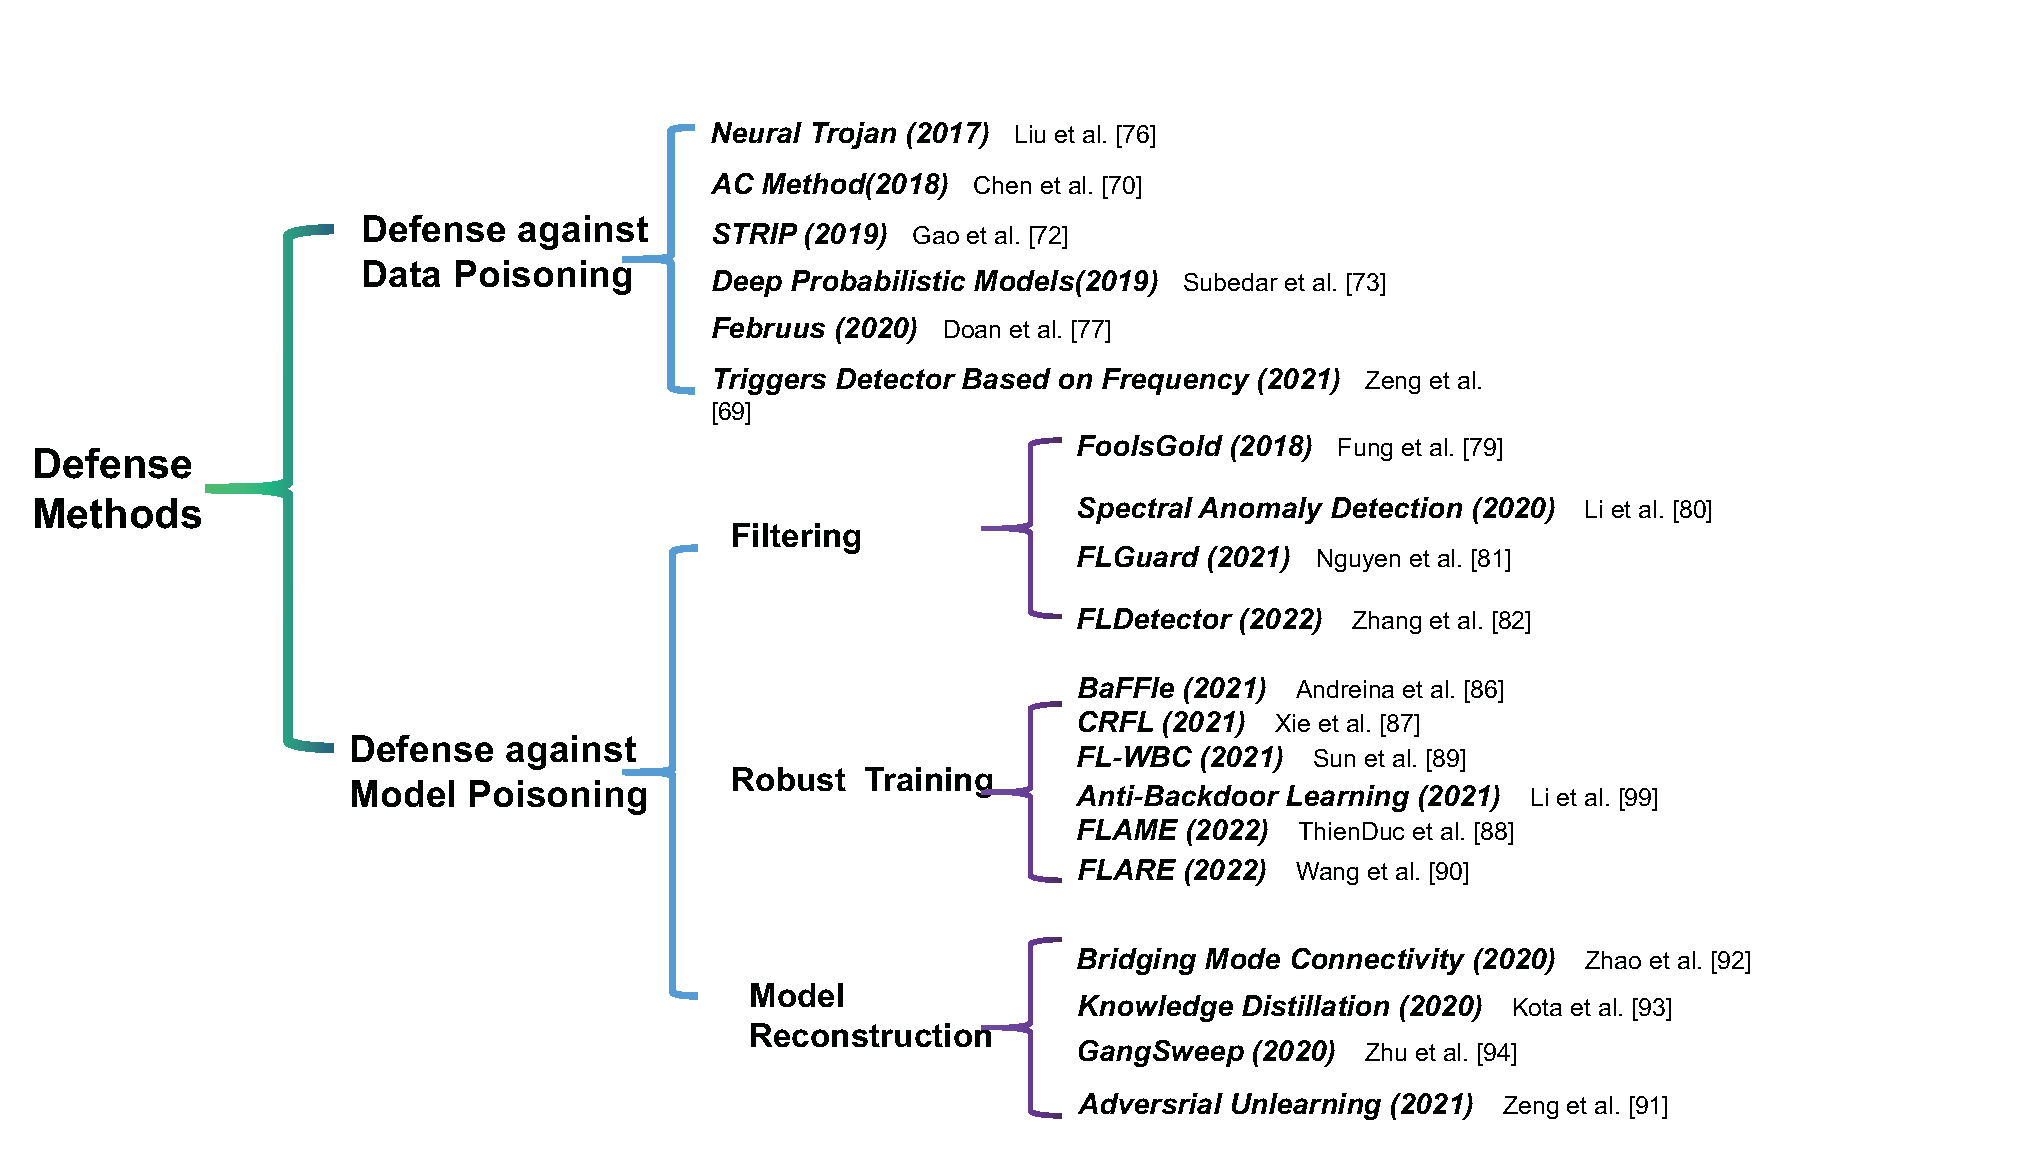
\includegraphics[width=1.0\linewidth,height=3.5in]{output/fig8.eps}
	\caption{This graph is a summary of some of the defensive solutions mentioned in this article, we have summarized and categorized some
		of them in this graph, and sorted them in chronological order.}
	\label{fig8}
\end{figure*}

To mitigate the problem of backdoor attacks in
federated learning, various defensive techniques have been
proposed. As shown in Fig.~\ref{fig8}, given that we previously
categorized backdoor attacks as data poisoning attacks
and model poisoning attacks, we will now discuss defensive
strategies for each of these attack types.

\subsection{Defense against Data Poisoning}
The simplest approach is to filter out poisoned data
samples, which aims to remove the poisoned samples from
the training datasets. After the filtering process, only
benign samples or purified poisoned samples are used
during the training process, thus eliminating the creation
of backdoors from the source.

Tran et al.~\cite{tran2018spectral} are the first to investigate methods
for filtering out malicious samples from the training sets.
They demonstrate that poisoned samples tend to leave
detectable traces within the covariance range of the feature
representation. Exploiting this insight, it is possible to
filter out poisoned samples from the training sets. Chen et
al.~\cite{chen2018detecting} propose a two-stage filtering approach. As shown
in Fig.~\ref{fig9}, in the first stage, activation values of samples
in each class are clustered into two groups. And in the
second stage, it is determined which clusters correspond
to poisoned samples. This method is the first methodology
for detecting poisonous data maliciously inserted into the
training set to generate backdoors that does not require
verified and trusted data. It has been released as a part
of the IBM Adversarial Robustness ToolBox. Similarly,
Zeng et al.~\cite{zeng2021rethinking} reveal that poisoned samples of existing
attacks have some high-frequency artifacts even if their
trigger patterns are invisible in the input space. Based on
this observation, they design a simple yet effective filtering
method based on those artifacts. Based on data-driven defense methods, in addition
to filtering out samples, it is also possible to consider
directly preprocessing the samples, specifically by erasing
any backdoors within them to prevent them from being
embedded in the model. Liu et al.~\cite{liu2017neural} propose a
pretrained autoencoder as a preprocessor to prevent malicious
samples from embedding backdoors by preprocessing the
input samples without affecting data classification accuracy.

Doan et al.~\cite{doan2020februus} propose a two-stage image processing
method called Februus, in which, in the first stage, Februus
uses GradCAM to identify influential regions, which are
then removed and replaced with neutral color frames.
Subsequently, as shown in Fig.~\ref{fig10}, Februus uses a GAN-based
repair method to reconstruct the masked regions
to mitigate their adverse effects (such as benign accuracy
reduction). Li et al.~\cite{li2021backdoor} discuss the properties of existing
poisoning-based static trigger mode attacks. They
demonstrate that the attack performance may sharply decrease
if the appearance or location of the trigger is slightly
changed. Based on this observation, they recommend using
spatial transformations (such as contraction, flipping) for
defense. Compared to previous methods, this method is
more efficient because it requires almost no additional
computational cost.

\subsection{Defense Against Model Poisoning}
(1)Filtering: Similar to defense methods against
poisoned data, defense methods against poisoned models also
begin with model filtering. Fung et al. propose FoolsGold~\cite{fung2018mitigating}
, which checks for and eliminates suspicious updates
during local updates. FoolsGold is based on the fact that
when a global model is trained by a group of attackers,
they will submit updates with the same backdoor objectives
throughout the training process, resulting in similar behaviors.

\begin{figure}[h]
	\centering
	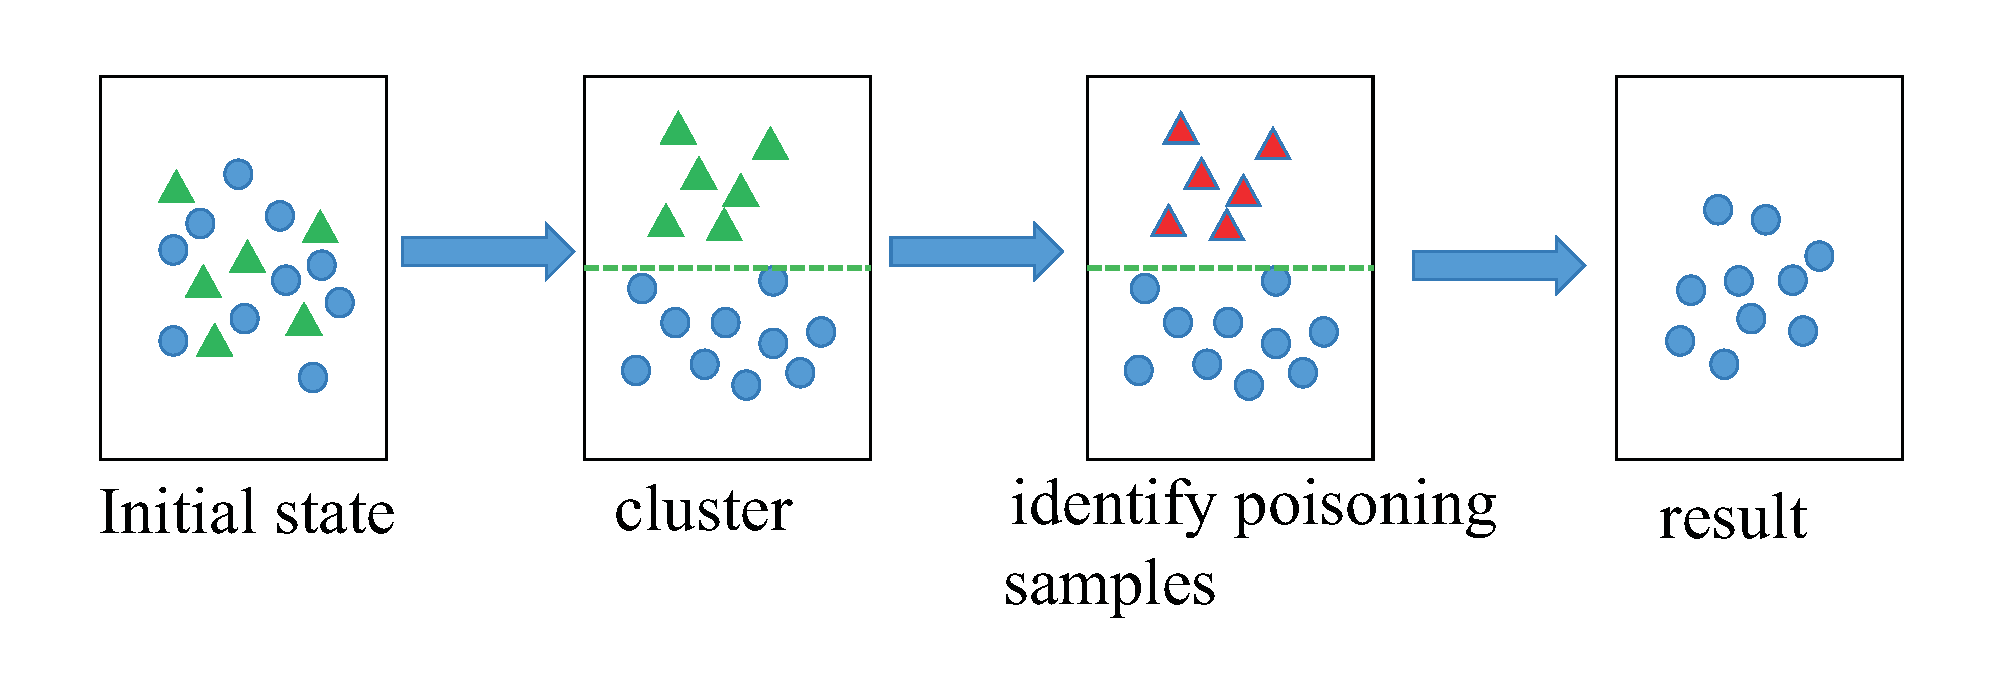
\includegraphics[width=1.0\linewidth,height=1.5in]{output/fig9.eps}
	\caption{In the first stage, activation values of samples in each class are
		clustered into two groups. And in the second stage, it is determined
		which clusters correspond to poisoned samples.}
	\label{fig9}
\end{figure}

However, this similarity does not occur among honest
participants because each user’s training datasets are
unique and not shared with others. Therefore,
malicious attackers can be separated from benign attackers
through gradient updates. After detecting such anomalies,
FoolGold maintains the learning rate of benign users
(submitting only unique gradient updates) and reduces
the learning rate of malicious users (repeatedly uploading
similar gradient updates) to mitigate backdoor attacks.
However, experimental results show that FoolsGold cannot
defend against adaptive attacks.

\begin{figure}[h]
	\centering
	\includegraphics[width=1.0\linewidth,height=2.2in]{output/fig10.eps}
	\caption{Februus uses a GAN-based repair method to reconstruct
		the masked regions to mitigate their adverse effects (such as benign
		accuracy reduction).}
	\label{fig10}
\end{figure}

Li et al.~\cite{li2020learning} propose a spectral anomaly detection
framework for a central aggregator that detects and
erases malicious updates through strong detection model
detection. The key idea of spectral anomaly detection
is that there is a significant difference between the
embedding of benign updates and backdoor updates in
a low-dimensional latent space. One practical method
for approximating low-dimensional embedding is to build
a model using an encoder-decoder structure, where the
encoder takes in the raw update and returns a low
dimensional embedding, and the decoder is fed the embedding and outputs the generation error.
After training the encoder-decoder model on benign updates, it can
be used to identify backdoor updates, generating errors
much higher than benign errors; malicious updates will
be excluded from the aggregation process. However, this
defense method cannot handle multi-trigger backdoor
attacks, i.e., injecting various backdoors simultaneously.

Nguyen et al. propose FlGuard~\cite{nguyen2021flguard}, a two-layer defense
method that checks for locally updated updates with
clear backdoor effects and eliminates residual backdoors
through pruning, smoothing, and noise addition. Unlike
FoolsGold~\cite{fung2018mitigating}, it also applies to multi-trigger backdoor
attacks while maintaining high prediction accuracy for
benign primary tasks. Additionally, FLDetector~\cite{zhang2022fldetector}
proposes a method to detect malicious clients by checking
the consistency of model updates. Essentially, the server
predicts the clien's model update based on past updates
in each iteration. If the model update received by the
client differs significantly from the predicted update over
multiple iterations, the client is marked as malicious.
Overall, the focus of these methods is mainly divided
into two types: the first is to remove toxic updates
from malicious clients before model aggregation, and the
second is to reduce the impact of malicious clients on the
aggregated model, such as reducing the learning rate of
suspicious clients.

(2)Robust Training: After filtering techniques, another
class of techniques aims to directly mitigate backdoor
attacks during model training through robust joint training.
Differential privacy algorithms have been shown to be
effective against backdoors~\cite{naseri2020toward}, but they may compromise
model performance under data imbalance commonly found
in federated learning~\cite{bagdasaryan2019differential}. DP-FedAvg~\cite{mcmahan2017learning} (Central-DP)
is a differential private aggregation strategy that
eliminates outliers by clipping the norm of model updates
and adding Gaussian noise, but the required amount of
noise significantly reduces task accuracy. Sun et al.~\cite{prakash2020mitigating}
proposed weak DP, which adds sufficient Gaussian noise to
defeat backdoors while maintaining task accuracy, but it is
ineffective against constraint-based backdoor attacks~\cite{li2023federated} .
Additionally, DP-based defenses can potentially impact
the benign performance of the global model, as the
clipping factor also changes the weights of benign model
updates.

In addition to DP-based defenses, Andreina et al.~\cite{andreina2021baffle}
propose Feedback-based Federated Learning (BaFFle)
to eliminate backdoors. The key idea of BaFFle is to
leverage participants to verify the global model. BaFFle
includes a super-digit verification process for each round
of federated learning. Specifically, each selected
participant checks the current global model by computing a
verification function on their secret data and reports to
the central server whether the model is backdoored or
not. The central server then decides whether to accept or
reject the current global model based on feedback from all
users. The verification function compares the error rate of
a specific class of the current global model with the error
rate of previously accepted global models. If the error
rate is significantly different, the central server rejects the
current global model as it may be backdoored and issues
an alert. Unlike anomaly detection, BaFFle is compliant
with secure aggregation.

\begin{figure}[h]
	\centering
	\includegraphics[width=1.0\linewidth,height=3.5in]{output/fig11.eps}
	\caption{Overview of certifiably robust federated learning (CRFL).
		CRFL controls the model smoothness through pruning and smooth-
		ing of model parameters and generates sample robustness certifica-
		tion against amplitude-limited backdoor attacks. Smoothness and
		perturbation methods are also used as additional components to
		constrain the L2 norm of individual updates to enhance defense
		performance.}
	\label{fig11}
\end{figure}

Considering that all of the above defense works lack
robustness certification, Xie et al.~\cite{xie2021crfl} propose the first
general defense framework CRFL for training certifiably
robust FL models against backdoor attacks. As shown
in Fig.~\ref{fig11}, CRFL controls the model smoothness through
pruning and smoothing of model parameters and generates
sample robustness certification against amplitude-limited
backdoor attacks. Smoothness and perturbation methods
are also used as additional components to constrain
the L2 norm of individual updates to enhance defense performance~\cite{nguyen2022flame}.
In addition, the FL-WBC~\cite{sun2021fl} method aims to identify
the fragile parameter space in FL and perturb it during
client training. FL-WBC also provides robustness
guarantees against backdoor attacks and convergence guarantees
for FedAvg. These developments demonstrate promising
steps toward improving FL's robustness against backdoor
attacks. In FLARE~\cite{wang2022flare}, a trust evaluation method is
proposed that calculates a trust score for each model
update based on the difference between all model updates
and their penultimate layer representation values. FLARE
assumes that most clients are trustworthy and assigns
low scores to updates that are far from benign update
clusters. The model updates are then aggregated with their
trust scores as weights and the global model is updated
accordingly. In~\cite{li2021anti}, the concept of anti-backdoor learning is
introduced, which involves training a clean model given
infected data, dividing the overall learning task into a
dual task of learning the clean part of the data and
the backdoor part. The article leverages two inherent
weaknesses of backdoor attacks: models learn backdoor
data faster than clean data, and the stronger the attack,
the faster the model converges on the backdoor data.
Additionally, backdoor tasks are mutually associated with
specific classes. Based on these two weaknesses, a generic
learning scheme is proposed to automatically prevent
backdoor attacks during training. A two-stage gradient
ascent mechanism is introduced to isolate and separate
backdoor samples from the target class during the early
training stage and break the association between backdoor
samples and the target class during the later training
stage.


(3)Model Reconstruction: The model reconstruction-based
approach aims to eliminate hidden backdoors in infected
models by directly modifying suspicious models.
Therefore, even if triggers are included in the attack
samples, the reconstructed model will still correctly predict
them because the hidden backdoors have been removed. As mentioned earlier, the forgetting mechanism of
federated backdoor attacks means that as training and
model aggregation progress, the backdoor will be forgotten
in successive iterations. As a defense, this forgetting
mechanism can also be utilized to create many defensive
methods. Zeng et al.~\cite{zeng2021adversarial} define multiple training as a min-max
problem and used implicit hyper-gradients to explain the
interdependence between internal and external optimization.
In~\cite{zhao2020bridging}, Zhao et al. show that hidden backdoors
infecting DNNs can be repaired using pattern connectivity
techniques with a certain number of benign samples. Li et al.~\cite{yoshida2020disabling} perturb backdoor-related neurons based
on the distillation process, reconstructed (infected) DNNs
using knowledge distillation techniques, and
thus removed hidden backdoors. Huang et al. ~\cite{huang2023distilling} propose a
distillation technique that utilizes Cognitive Distills to
extract Cognitive patterns. This is because the patterns of
backdoor examples are generally small and sparse, making
it possible to detect poisoned examples.

In addition to directly eliminating hidden backdoors,
defense based on trigger synthesis first synthesizes
backdoor triggers, and then in the second phase, eliminates
hidden backdoors by suppressing the influence of triggers.
These defenses have some similarities in the second phase
with reconstruction-based defenses. For example, pruning
and retraining are commonly used techniques to remove
hidden backdoors in both defenses. However, compared to
reconstruction-based defenses, the trigger-based defenses'
trigger information makes the removal process more effective and efficient.

A GAN-based method is proposed in~\cite{zhu2020gangsweep} to synthesize
trigger distributions. In~\cite{guo2020towards}, they show that the detection
process used in~\cite{wang2019neural} to determine synthesized triggers has
several failure modes and proposed a new defense method
based on this observation. Additionally, Cheng et al. ~\cite{xu2020defending}
reveal that the $\infty$ norm of activation values can be used to
distinguish backdoor-related neurons based on synthesized
triggers. Therefore, they propose performing an $\infty$-based
neuron pruning to remove neurons with high activation
values in response to triggers. Similarly, Aiken et al.~\cite{aiken2021neural}
also propose removing hidden backdoors by pruning DNNs
based on synthesized triggers from another perspective.

In general, we do not consider filtering techniques to be
a viable solution for mitigating backdoor attacks. Because
filtering technologies are generally designed for specific
types of attacks, they can be easily spoofed by attackers.
Instead, we believe that the focus of research on backdoor
defense should be on model reconstruction and robust
training.


\section{Byzantine Attack}
The Byzantine attack is a malicious attack that
typically occurs in distributed systems with malicious
participants. In the field of computer science and cryptography,
the Byzantine Generals Problem describes the scenario
of distributed systems with malicious participants. The
essence of the Byzantine Generals Problem lies in how
to achieve consensus among all nodes in the system
when facing potential malicious participants. Byzantine
attacks pose a significant threat to the security and
reliability of distributed systems. This chapter focuses
on categorizing Byzantine attacks into three types and
provides an overview of the challenges faced and future
directions for development. As shown in Fig.~\ref{fig13}, we will
analyze Byzantine attack from 3 aspects.

\begin{figure*}[htbp]
	\centering
	\begin{minipage}{0.49\linewidth}
		\centering
		\includegraphics[width=1.0\linewidth,height=2.5in]{output/fig12.eps}
		\caption{The schematic of defense methods of Byzantine attack.}
		\label{fig12}
	\end{minipage}
	% \vspace{-0.2cm}
	\begin{minipage}{0.49\linewidth}
		\centering
		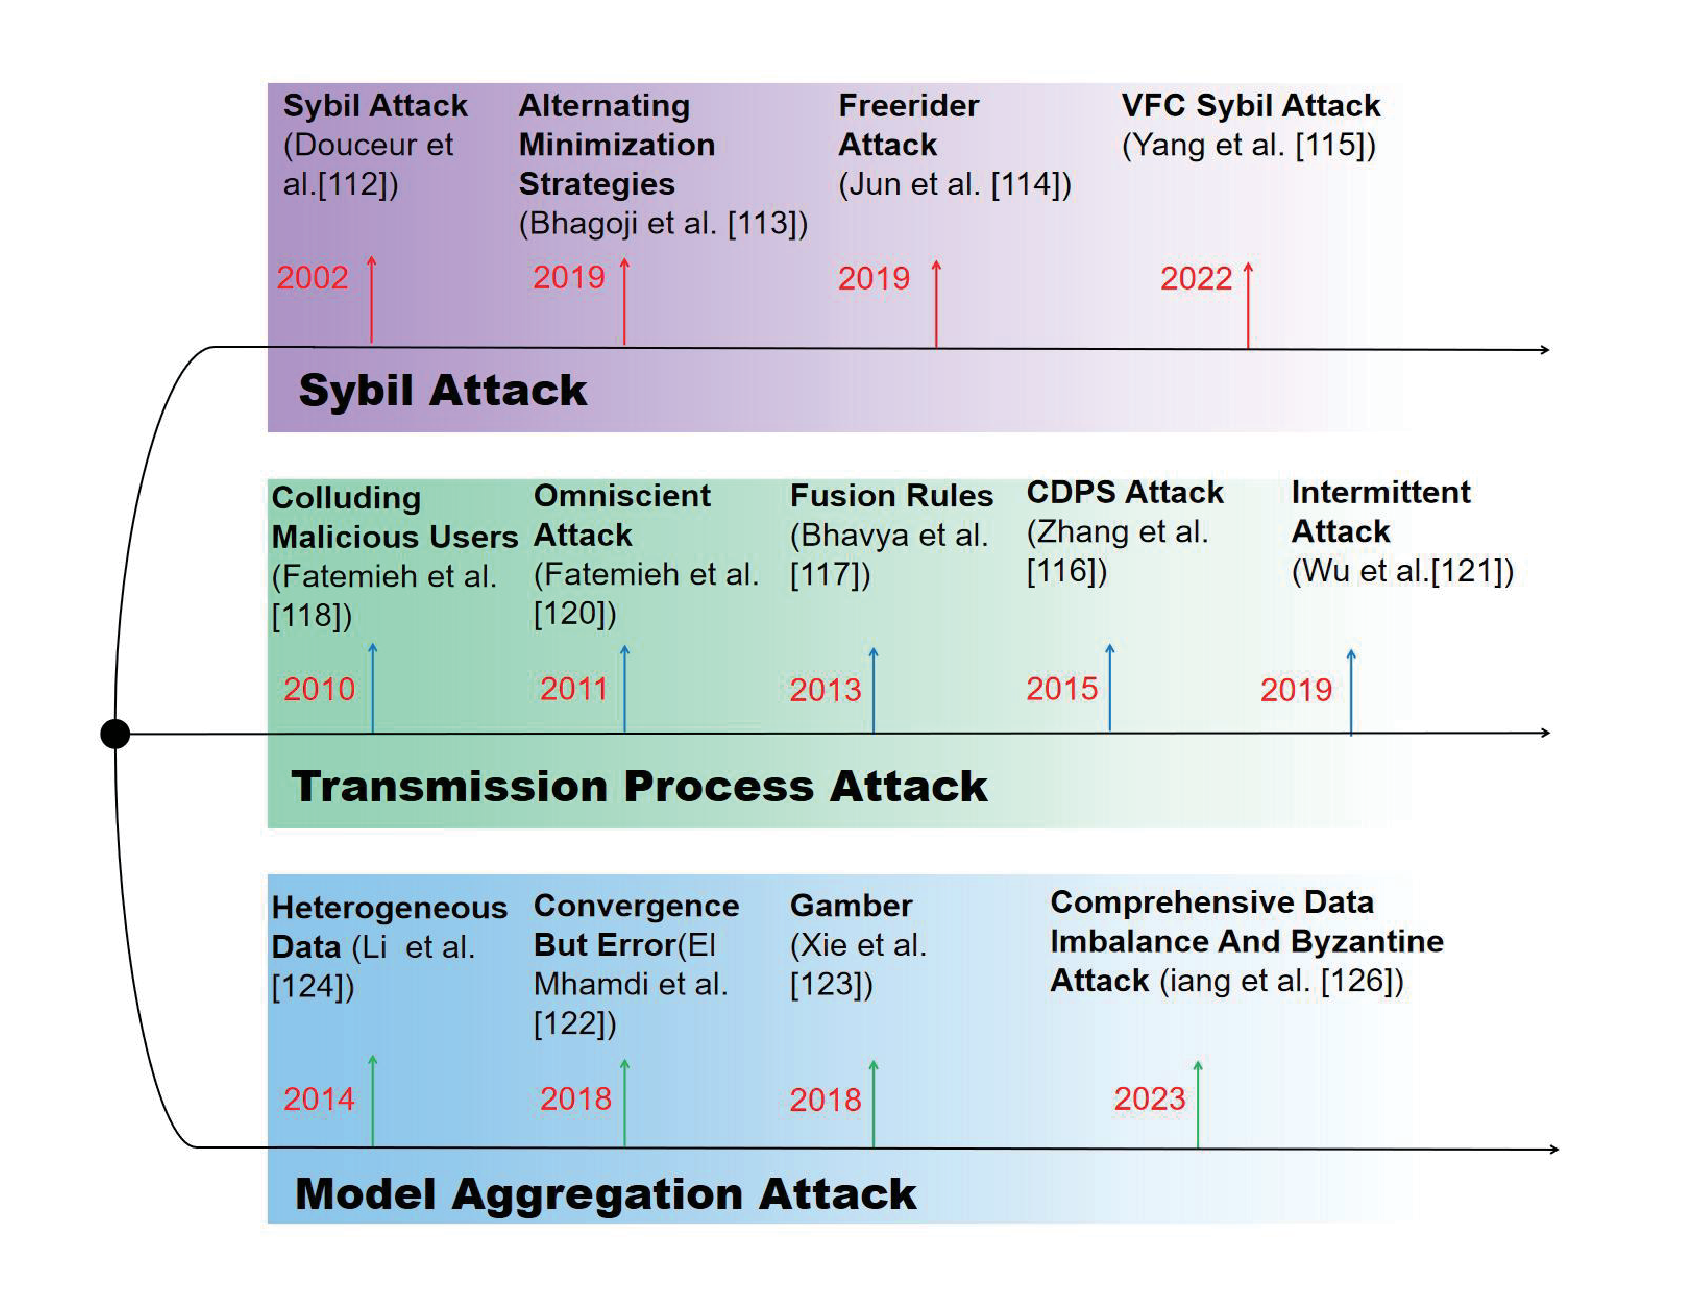
\includegraphics[width=1.0\linewidth,height=2.5in]{output/fig13.eps}
		\caption{The schematic of Byzantine attack.}
		\label{fig13}
	\end{minipage}
\end{figure*}



\subsection{Sybil Attack}
\begin{figure}[h]
	\centering
	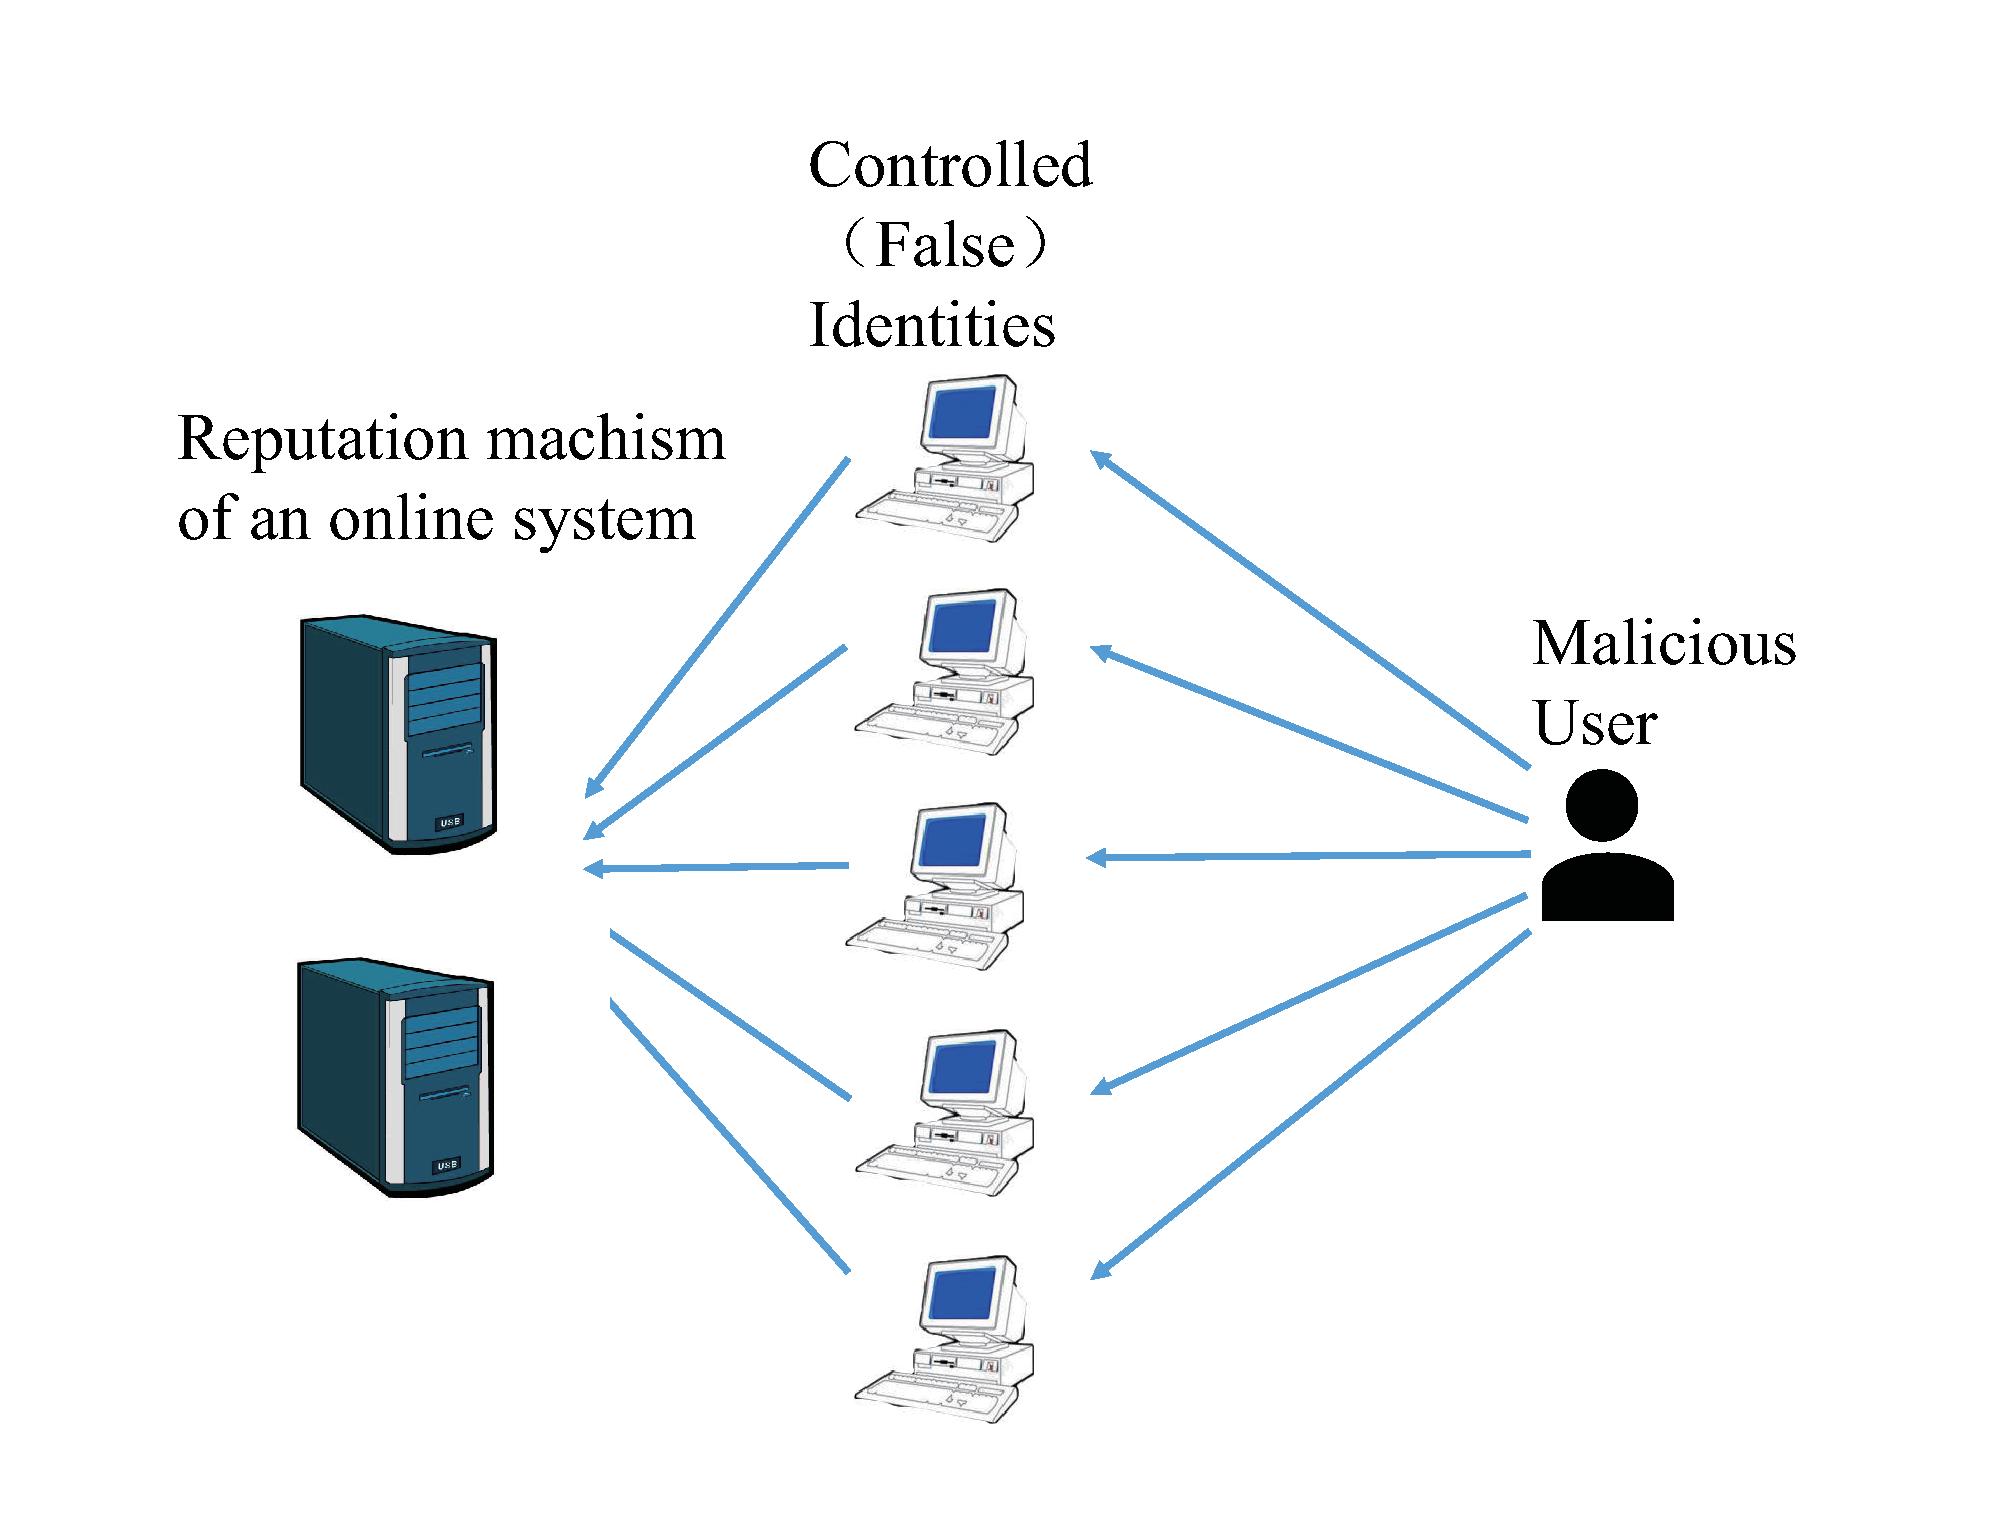
\includegraphics[width=1.0\linewidth,height=3.5in]{output/fig14.eps}
	\caption{The schematic of the Sybil attack. Malicious users create a
		large number of fake nodes and control them to disrupt the normal
		operation of the network.}
	\label{fig14}
\end{figure}

The first type of Byzantine attacks is the Sybil attack.
It was first proposed by John Douceur et al. in 2002~\cite{douceur2002sybil}
. As shown in Fig.~\ref{fig14}, it is a type of network security
attack where the attacker creates multiple fake identities
or nodes to undermine the network's trust mechanism and
disrupt its normal operation. The principle behind this
attack is that the attacker creates a large number of fake
identities, nodes, or accounts that appear independent and
genuine to the network but are actually controlled by the
attacker. The attacker can use various means to create
these fake entities, including using forged IP addresses,
anonymous proxy servers, virtual machines, and more.
This attack mainly targets systems that rely on trust
and identity verification mechanisms, such as
peer-to-peer networks, social networks, and blockchains. Attackers
can use a large number of fake identities to control the
resources of the system, deceive other users, and disrupt
consensus mechanisms. For example, in a peer-to-peer
network, attackers can create numerous fake nodes to
control the distribution process of files, leading to uneven
resource distribution or network performance degradation.


The Sybil attack has posed significant threats to various
network security systems since it was proposed. Bhagoji
et al.~\cite{bhagoji2019analyzing}, Jun et al. ~\cite{lin2019free} and Yang et al.~\cite{yang2022overview} explore
it from the aspects of attack strategy, attack form and
attack field respectively. Bhagoji et al.~\cite{bhagoji2019analyzing} explore some
attack strategies against deep neural networks by
enhancing malicious agent updates and employing alternating
minimization strategies for stealth and adversarial targets.
They demonstrate the possibility of effective and covert
model poisoning attacks. Jun et al.~\cite{lin2019free} are the first
to explore the Freerider attack in federated learning and
propose an incremental weight attack method that can
evade most defense monitoring methods at that time. They
also introduce a new high-dimensional anomaly detection
method called STD-DAGMM, which is particularly useful
for detecting freeriders. This method has potential
applications for detecting other models' weight anomalies as well,
which will be discussed in the next chapter. Yang et al.~\cite{yang2022overview}
focus on the problem of vehicular ad hoc networks
and criticized previous studies for only considering the
security threats and impacts of Sybil attacks in VANETs
without analyzing the potential threats and impacts in
VFCs (Vehicular Fog Computing). Therefore, the authors
summarize four types of Sybil attacks that could affect
VFCs in areas such as routing, vehicle decision-making,
voting, and reputation systems.

In recent years, Sybil attacks have undergone significant
development. Attackers employ more advanced techniques
to create false identities, making Sybil nodes more realistic
and difficult to distinguish. For instance, they may use
virtualization technology to create multiple independent
virtual machines, each with its own IP address and
network identifier. Attackers can also utilize social
engineering tactics and information acquisition methods to disguise
themselves as genuine users or obtain additional fake
identities through the authorization of legitimate users.
Furthermore, attackers might construct more complex and
realistic Sybil networks by leveraging shared information
in social networks. With the widespread use of mobile
devices and the wireless networks, Sybil attacks have also
started to increase in these environments. Attackers can
threaten the security of location services, social networks,
and mobile applications by utilizing false identities and
location information on mobile devices. In the future, Sybil
attacks can be more extensively applied to blockchain
technology, which enable attackers to manipulate
consensus algorithms, launch double-spending attacks, or
undermine the fairness of blockchain networks by controlling a
large number of counterfeit identities.

\subsection{Transmission Process Attack}
The second type of Byzantine attacks is based on
the transmission process. Byzantine attacks can occur
during the communication process between participants. Attackers can tamper with, delete, or insert malicious
messages to disrupt the transmission of model updates.

Zhang et al.~\cite{zhang2015byzantine} propose a centralized related
probability small-scale attack (CDPS), which utilizes additional
information. For instance, fusion rules in fault diagnosis~\cite{kailkhura2013distributed}
can be considered as existing knowledge usable
for optimizing attack tactics. One form of CDPS attack
involves collaborative efforts among malicious users who
engage in communication. Moreover, sharing of
information can assist malicious users in devising efficient attack
strategies. Generally, colluding malicious users~\cite{fatemieh2010secure,qin2013defending}
first exchange measurement values to ensure more accurate
decisions on the licensed channel state and then report
the coordinated forged results to enhance attack power.
Moreover, Fatemieh et al.~\cite{fatemieh2011using} introduce another attack
model called the full-knowledge attack.

Cooperative spectrum sensing (CSS) is considered a
promising method for identifying available spectrum.
However, it not only requires a significant amount of
communication resources but also introduces vulnerabilities to
Byzantine attacks. Wu et al.~\cite{wu2018sequential} mention that attackers
keep reporting false information to the fusion center
consistently. In fact, attackers may attack discontinuously
while appearing normal during rest periods. The authors
propose a low-complexity sequential 0/1 (S0/1) method
for CSS in the presence of strategic Byzantine attacks.
It does not require strong assumptions or any prior
knowledge, and this method will be discussed in the next
chapter.

With the development of IoT devices, attackers may
exploit communication vulnerabilities and weaknesses
between IoT devices to launch future attacks. Attackers may
also utilize high-speed, low-latency 5G/6G networks to
carry out large-scale distributed denial-of-service (DDoS)
attacks, bypass security measures using network slicing
and virtualization technologies, or exploit vulnerabilities
in mobile communication protocols to attack devices and
systems.

\subsection{Model Aggregation Attack}
The third type of Byzantine attacks is known as model
aggregation attack. In this type of attack, Byzantine
attackers manipulate the model parameters of the
participants in order to influence the aggregation results.

\begin{figure}[h]
	\centering
	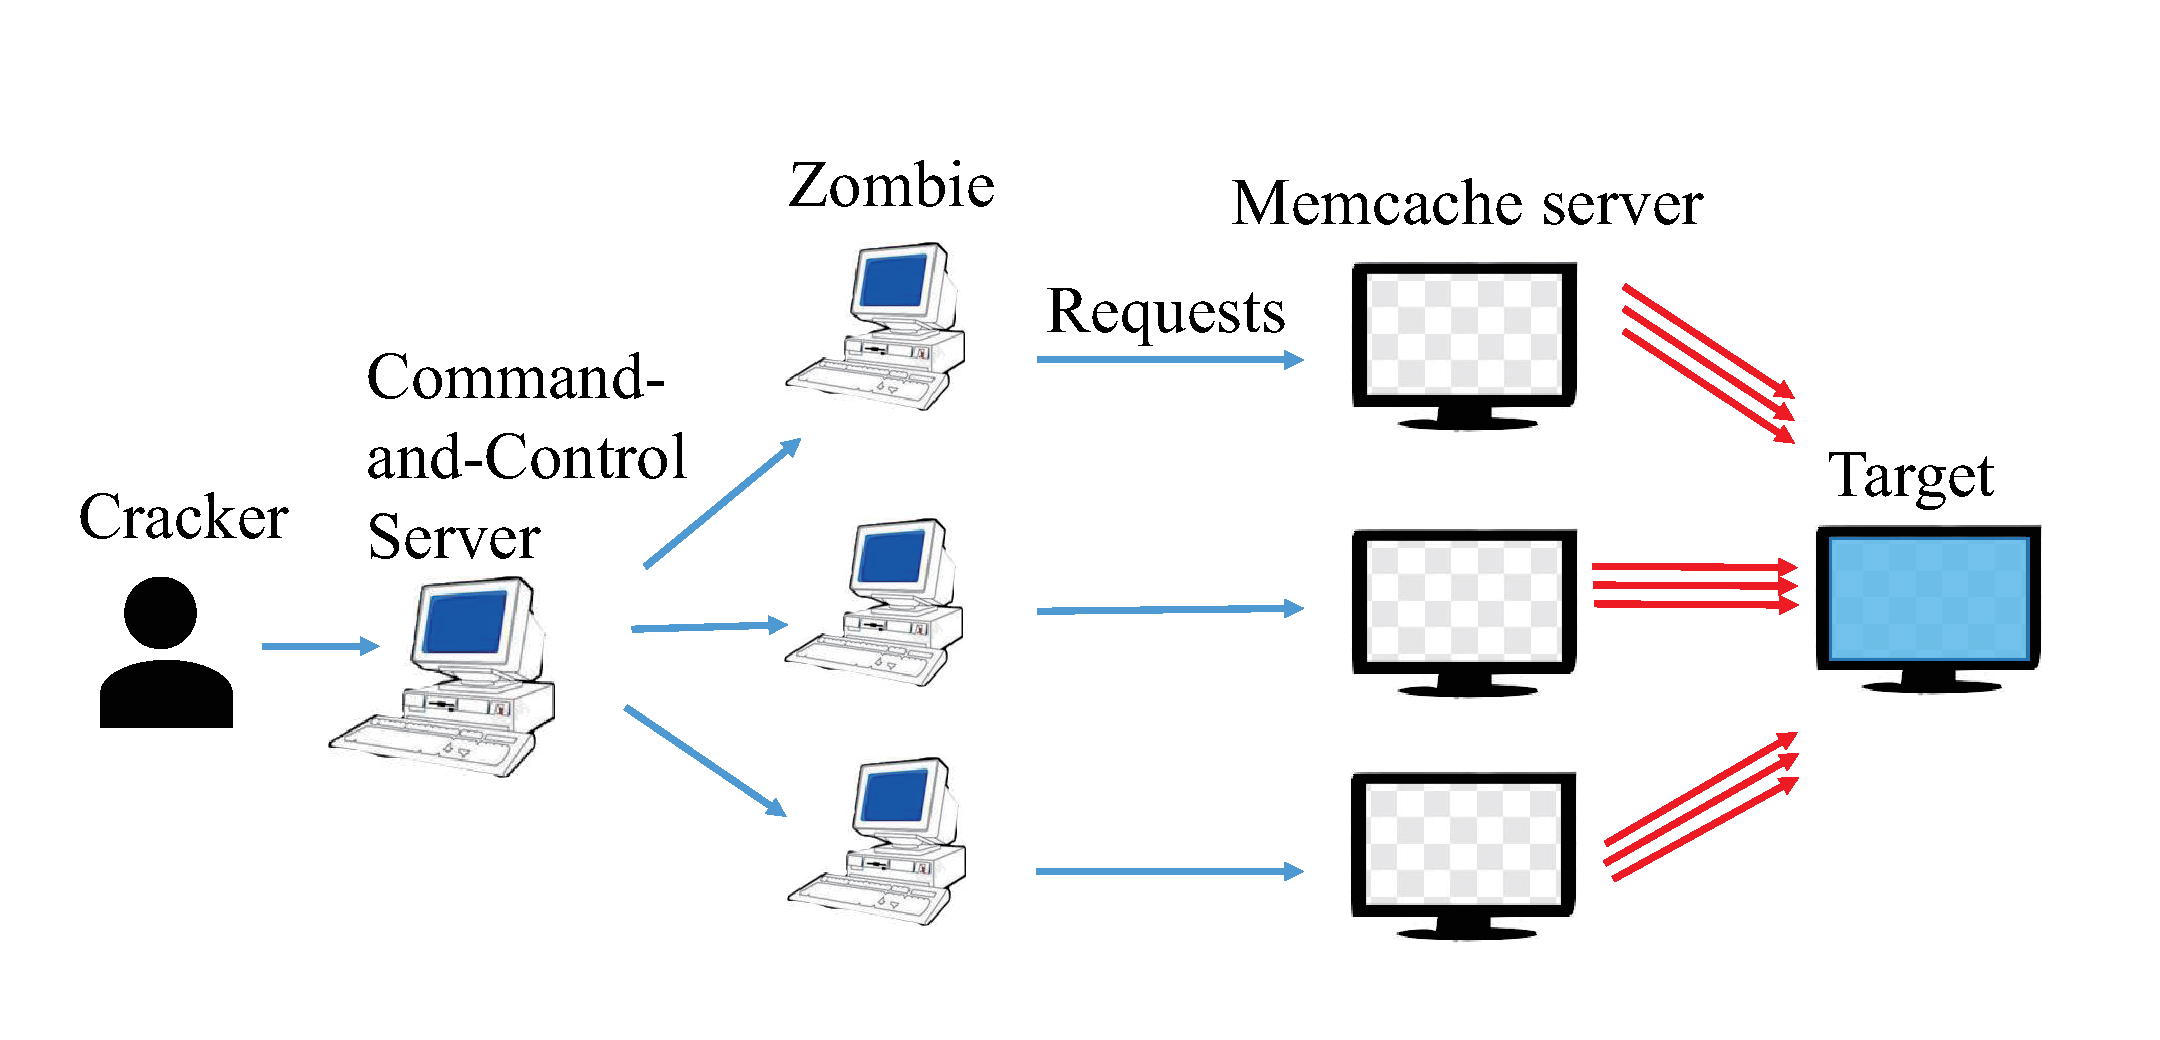
\includegraphics[width=1.0\linewidth,height=2.5in]{output/fig15.eps}
	\caption{The schematic of a DDOS attack. Through the central
		control system, the attacker uses specific software or malicious code
		to remotely control multiple zombies, making them send a large
		number of requests to the target system at the same time to exhaust
		the processing power, network bandwidth or resources of the target
		system, thus causing the target system to fail to work normally.}
	\label{fig15}
\end{figure}

As discussed by El Mhamdi et al.~\cite{guerraoui2018hidden}, these attacks by
Byzantine workers may not prevent the model from
converging but can instead lead to convergence on suboptimal
solutions. This is a new way of thinking and there is a lot of
room for development in the future. However, most attacks
disrupt the convergence of the model. Xie et al.~\cite{xie2018generalized}
propose a form of attack called Gamber. In this attack,
an attacker can modify some of the data communicated
between participants. The attacker randomly selects data
and makes malicious changes to them. The authors also
mention several other attacks,such as omniscient. The
attacker needs to have knowledge of the gradients sent by
all the staff members and replaces some gradient vectors
by taking the sum of all gradients, scaled by large negative
values. The objective is to mislead the Stochastic Gradient
Descent (SGD) algorithm into moving in the opposite
direction with larger step sizes. Weaker attacks, such as
Gaussian attacks, are also possible.In these attacks, some
gradient vectors are replaced with random vectors sampled
from a Gaussian distribution that has a large variance.
Such attackers do not require any information from the
staff members.

\begin{figure}[h]
	\centering
	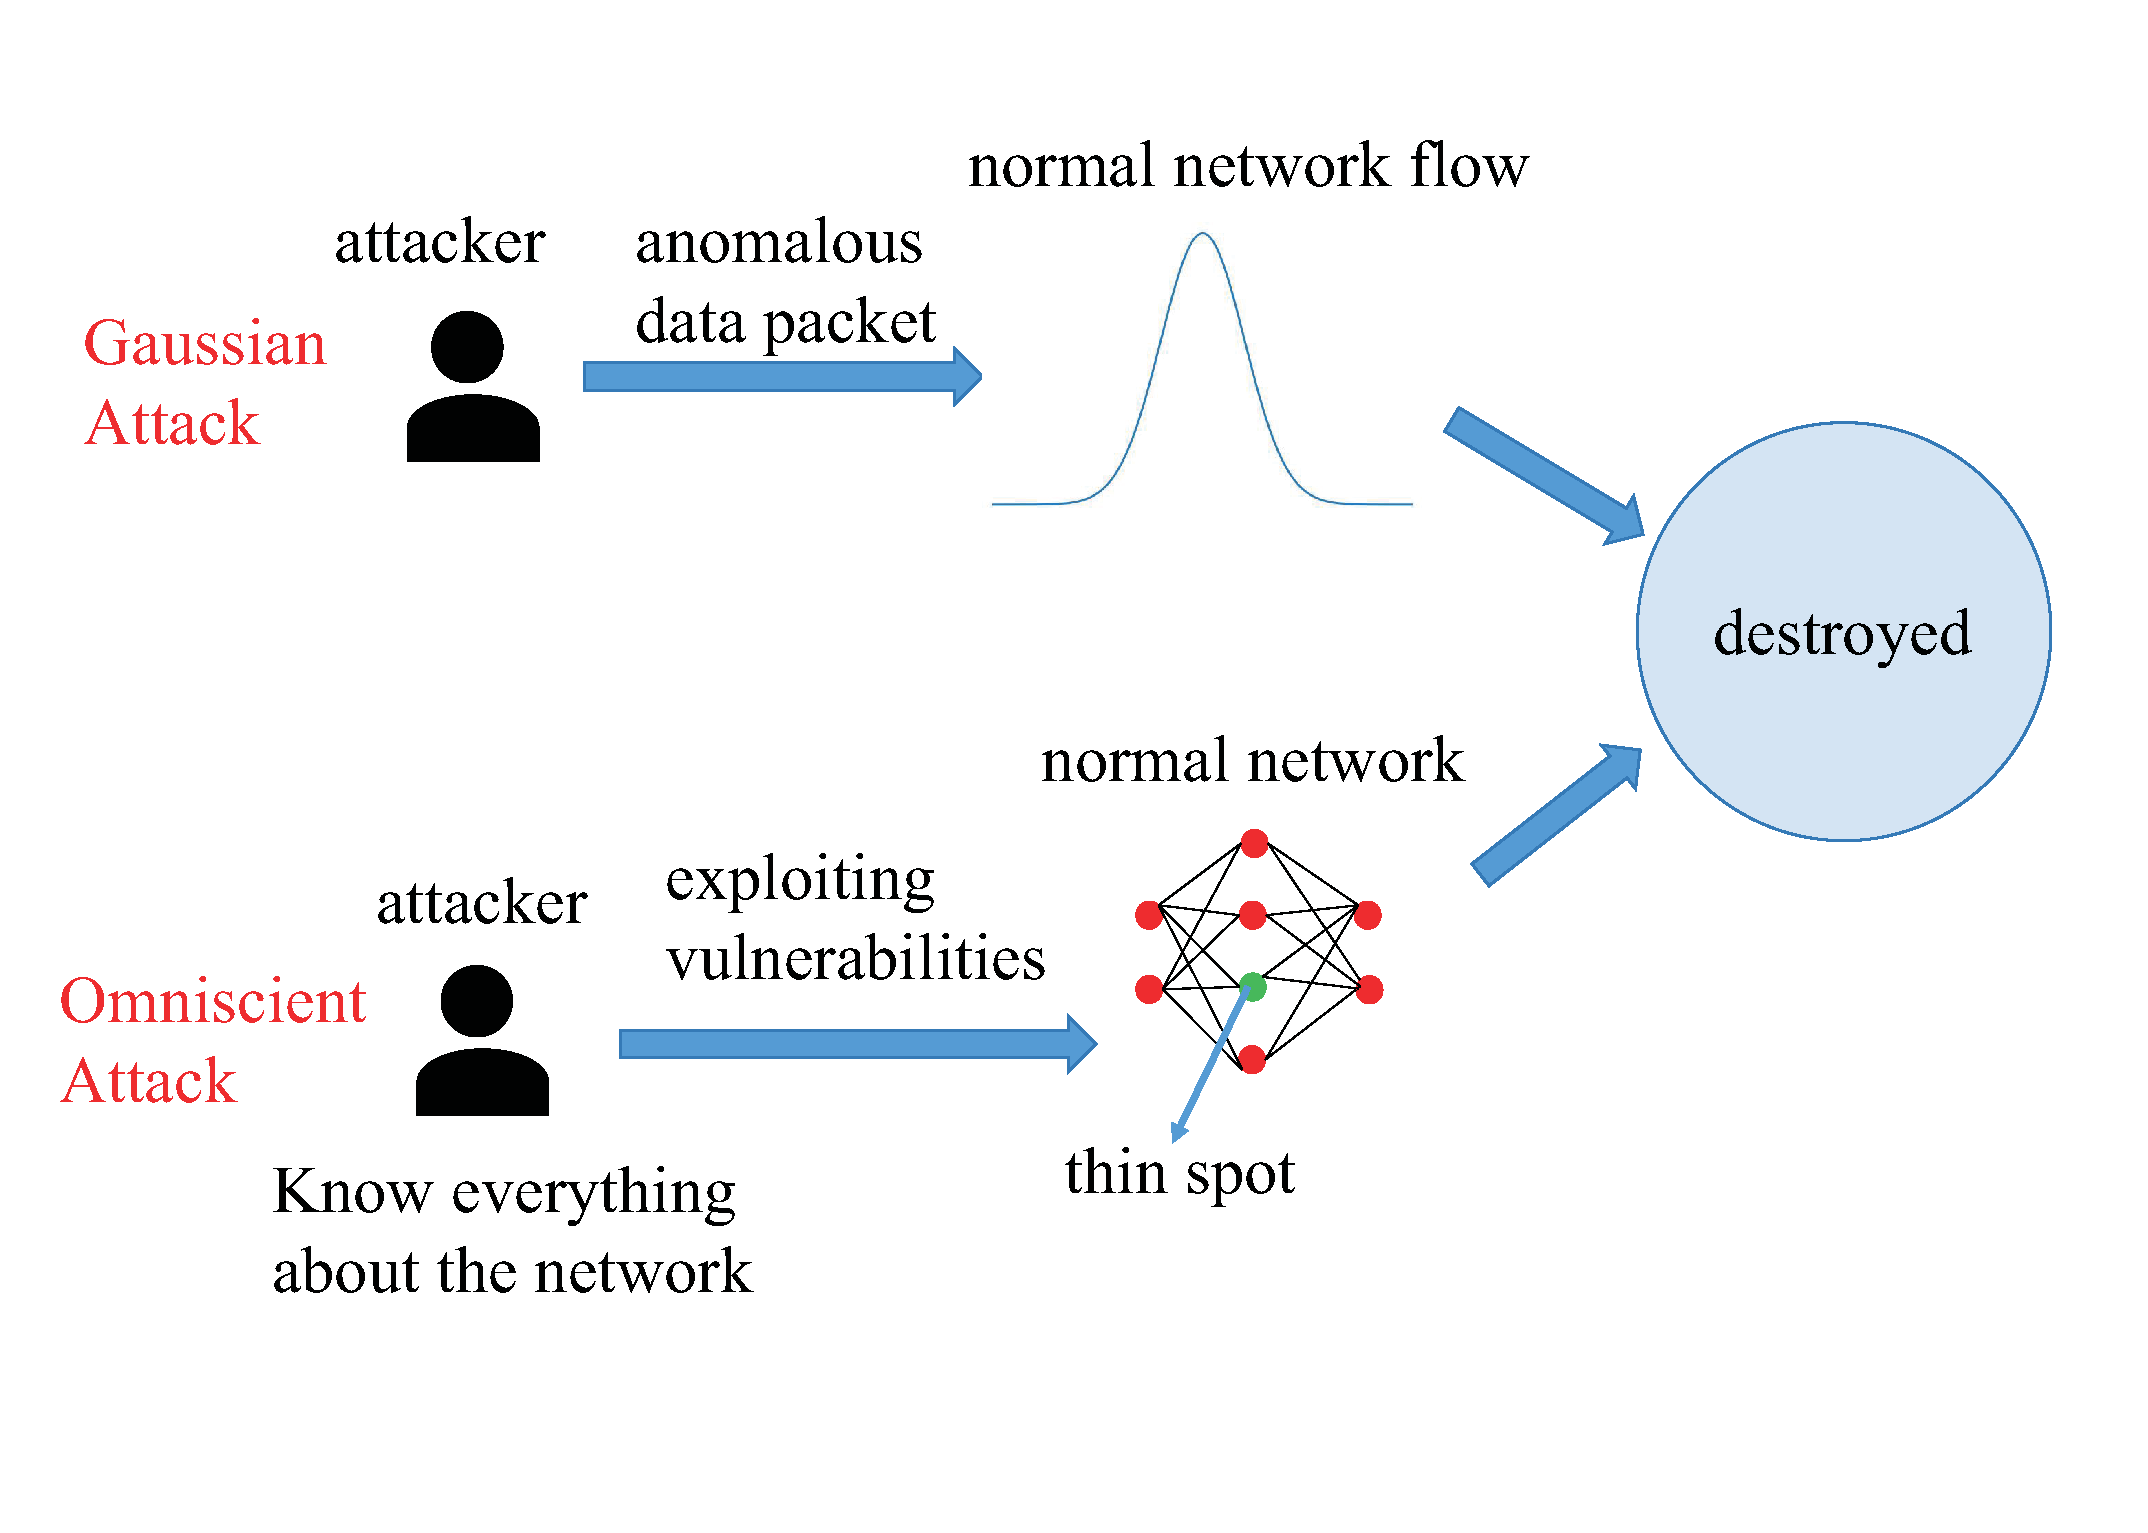
\includegraphics[width=1.0\linewidth,height=3.5 in]{output/fig16.eps}
	\caption{The schematic of Gaussian attack and Omniscient attack.In
		a Gauss attack, an attacker enters incorrect packets into the network,
		affecting the normal running of network flows.An omniscient attack is
		a hypothetical scenario where an adversary has complete and perfect
		knowledge or awareness of the system they are targeting. In this
		type of attack, the adversary has access to all the information and
		capabilities necessary to exploit vulnerabilities in the system. With
		this all-encompassing knowledge, the attacker can strategically plan
		and execute attacks to maximally exploit the system’s weaknesses.}
	\label{fig16}
\end{figure}


In many applications, multiple sources can provide
descriptions of the same object or event, which can inevitably
lead to conflicts in data or information. Resolving conflicts
in data is an important challenge in achieving convergence
in federated learning. Byzantine attackers have the ability
to exploit these issues in order to manipulate the
convergence of the model. Li et al.~\cite{li2014resolving}, Hsu et al.~\cite{hsu2019measuring}, and
Jiang et al.~\cite{jiang2023secure} have all explored questions related to
data differences and conflicts.

In future attacks, attackers may attempt to achieve their
objectives by making modifications to the trained model.
This can involve incorporating backdoors into the model,
which would produce incorrect outputs under specific
conditions, or tampering with the model parameters to
disrupt its robustness. In order to evade detection, future
attack strategies could involve the development of more
advanced and covert techniques to camouflage malicious
modifications. Additionally, malicious insiders who have
access to the model parameters may exploit this privilege
to launch attacks. They could manipulate the parameters
to compromise the model's performance or even insert
sensitive information within the model itself. In the coming
years, attackers may explore more complicated techniques
and algorithms to bypass security monitoring and
detection mechanisms. The aim would be to implement internal
personnel attacks more efficiently. These advancements
would allow attackers to bypass existing safeguards and
carry out their malicious activities with greater precision
and effectiveness.

\section{Defenses Against Byzantine Attack}
With the advancement of Byzantine attacks, the
corresponding defense methods are constantly evolving and
being updated. As shown in Fig.~\ref{fig12}, based on the different
types of Byzantine attacks discussed in the previous
chapter, we categorize the Byzantine defense methods into
three classes:

\subsection{Defenses against Sybil Attack}
For Sybil attacks, the defense methods include trust-based
evaluation methods and machine learning models
for detecting fake nodes. Gil et al.~\cite{gil2017guaranteeing} propose a novel
algorithm that analyzes received wireless signals to detect
the presence of deceptive clients created by adversaries.
It does not require specialized hardware or private key
exchanges, commercial Wi-Fi cards and software are
enough. It utilizes the physical characteristics of wireless
signals to ”perceive” deceivers. The authors conduct
experiments using the AscTec quadcopter server team and
iRobot Create ground clients, which show a deception
detection rate exceeding 96Blanchard et al.~\cite{blanchard2017machine} introduce
Krum, which detects and removes outliers in gradient
aggregation, allowing convergence even in the presence
of multiple Byzantine attackers, and with low complexity.
Gil et al.~\cite{gil2017guaranteeing} and Blanchard et al.~\cite{blanchard2017machine} reduce the impact
of the attacker, but don't accurately detect the attacker
and remove it.

\begin{figure}[h]
	\centering
	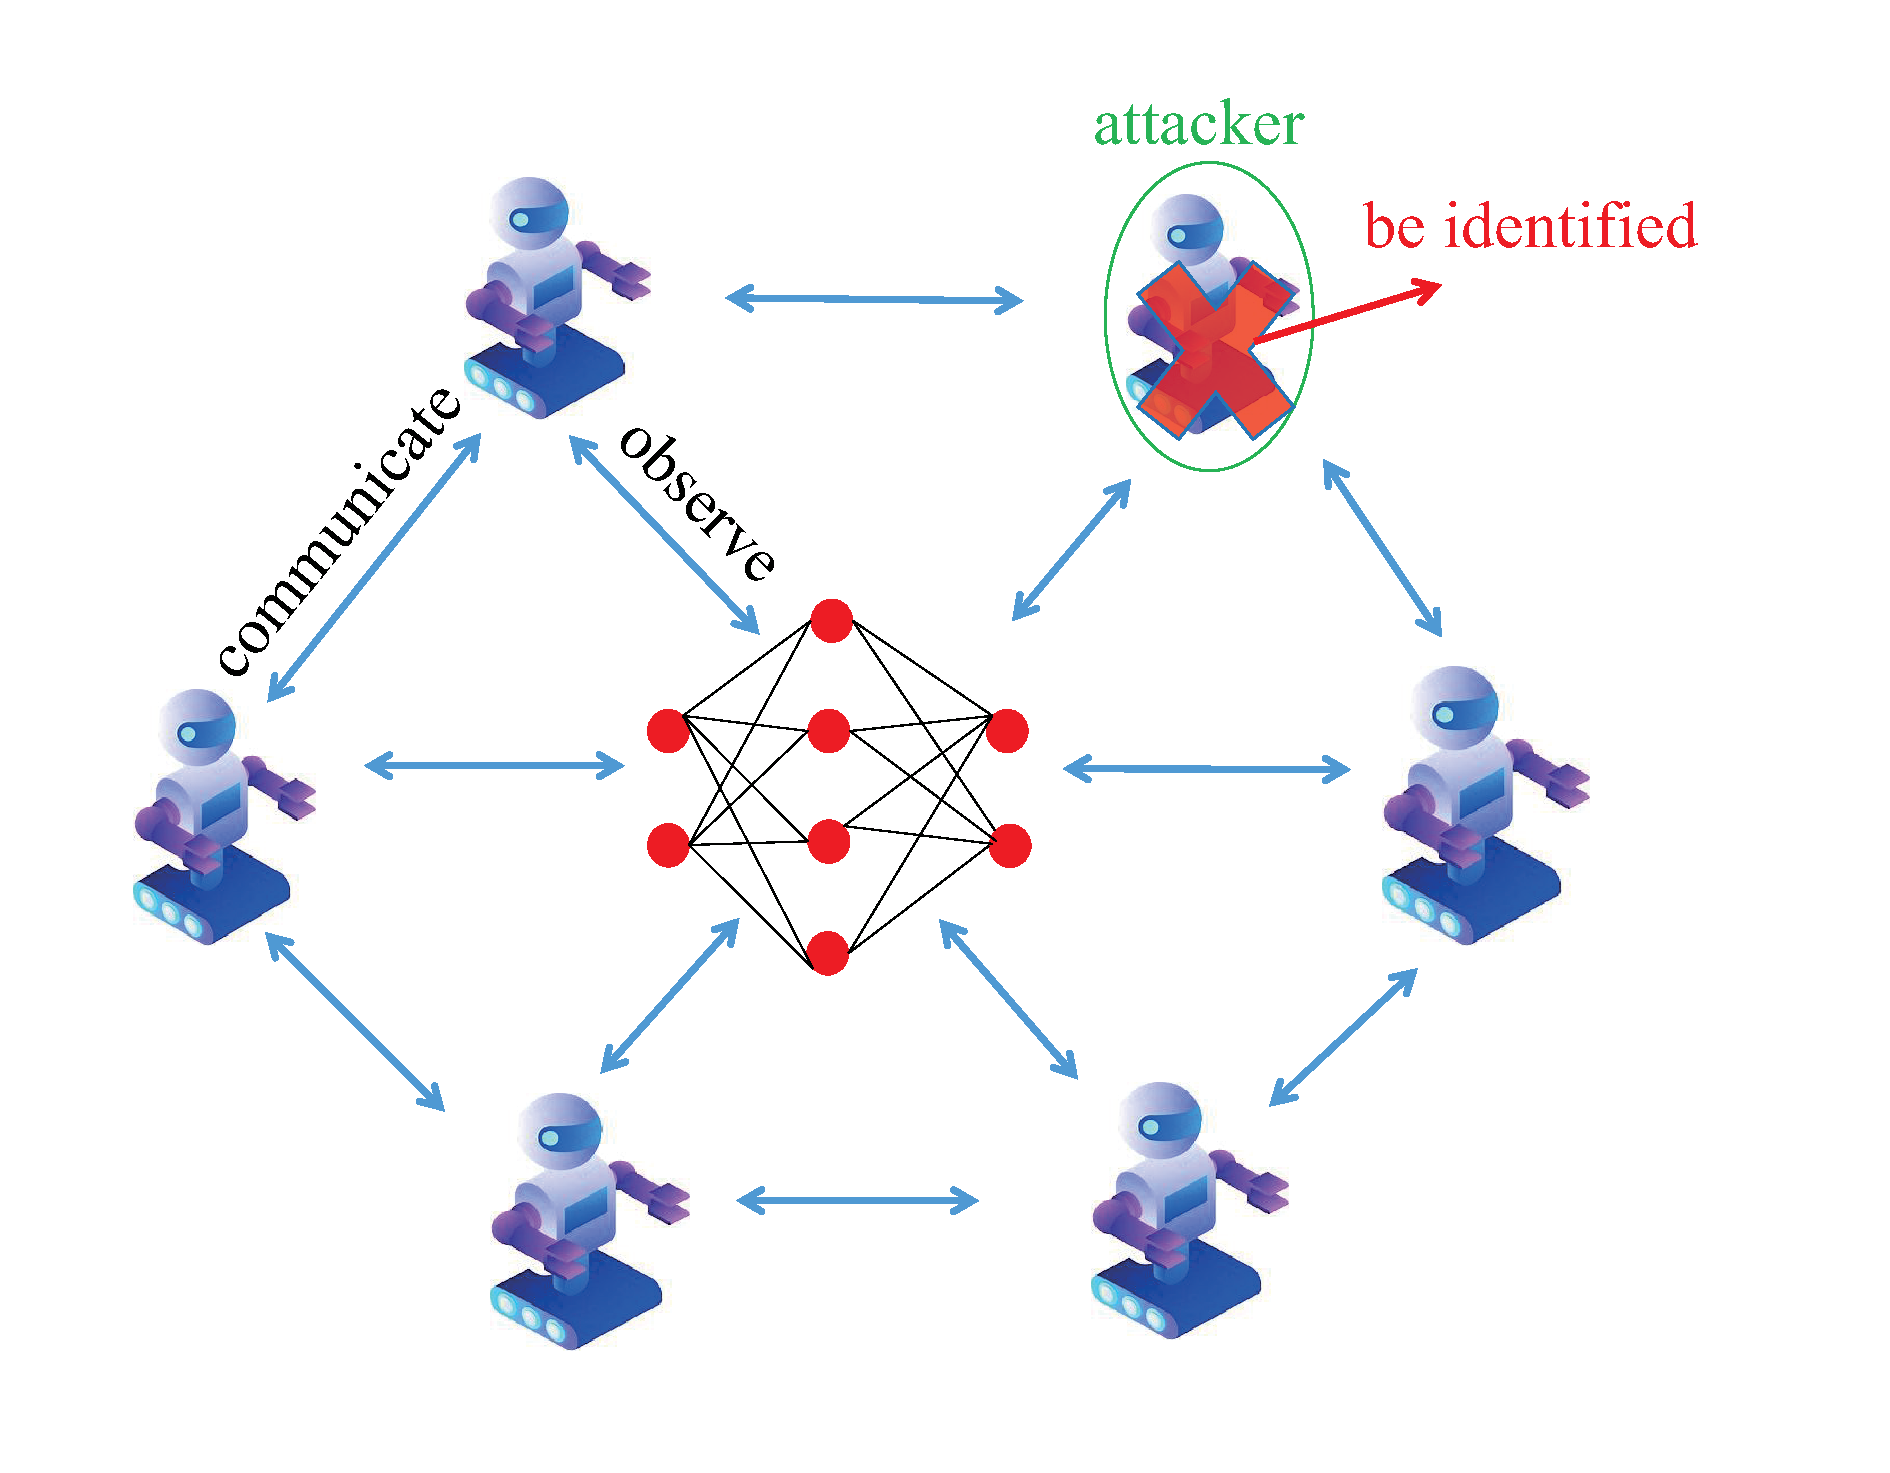
\includegraphics[width=1.0\linewidth,height=3.5in]{output/fig17.eps}
	\caption{Robots can communicate with neighbors to get information,
		combined with their own information, in a certain round can
		eliminate the interference of malicious robots, reach a consensus.}
	\label{fig17}
\end{figure}


Both of the following methods detect the malicious
attacker and remove its effects. Muñoz-González et al.~\cite{munoz2019byzantine}
propose a new algorithm for robust federated learning
called Adaptive Federated Averaging, aims to detect
faults, attacks, and malicious updates provided by
participants in a collaborative model. The authors also propose
a Hidden Markov model to simulate and learn the quality
of model updates provided by each participant during
training. In the work of Mallmann-Trenn et al.~\cite{mallmann2021crowd}, a
combination of wireless signal analysis and observations
from sociological learning is used to demonstrate rapid
convergence of correct trust values for all robots in the
team when facing attacks. All robots develop their own
opinions about network trust by observing messages sent
through the network as shown in Fig.~\ref{fig17}. They compare
their opinions with those of their neighbors to reach
a consensus on whether the robots can be trusted. By
utilizing their neighbors' opinions, each robot effectively
increases the number of observations available to them
about the network, thereby eliminating messages with a
high probability of coming from malicious robots through
cross-validation. Experiments show that in a limited
number of communication rounds, all robots agree on the
global consensus of trustworthiness in their neighborhood.

Sybil attacks pose a significant challenge as attackers
can create a large number of false identities, making it
difficult to detect and differentiate them. Therefore,
developing secure systems requires consideration of multiple
defense methods and selecting appropriate solutions based
on specific application contexts. The future outlook for
such defense techniques primarily focuses on the following
areas: enhancing identity verification mechanisms to
distinguish genuine users from Sybil nodes and establishing
stronger trust mechanisms to identify and filter out Sybil
nodes displaying malicious behavior. In recent years,
the emergence of blockchain technology has provided a
decentralized, tamper-resistant, and secure shared ledger,
offering a potential defense against Sybil attacks. By
combining identity verification, trust mechanisms, and
blockchain technology, the ability to detect and prevent
Sybil nodes can be improved.

\subsection{Defense Against Transmission Process Attack}
Defense methods against attacks during the transmission
process include designing secure communication
protocols and encryption mechanisms. Previous malicious detection and suppression
algorithms focused only on simple ”always attack” scenarios,
where attackers continuously report false information to
the central entity. In reality, attackers may intermittently
attack while behaving normally at other times. Under the
assumption of simple attack strategies, Chen et al.~\cite{chen2012robustness}
propose sequential hypothesis testing to defend against
Byzantine attacks, but it requires significant
computation and prior knowledge. Therefore, Wu et al.~\cite{wu2018sequential}
introduce S0/1 using support vector regression (SVR)
to offset strategic Byzantine attack defense. Even in a
blind scenario, this approach greatly reduces the sample
size while providing higher correct sensing ratios.
MuñozGonzález et al.~\cite{munoz2019byzantine} also propose a robust aggregation
rule that detects and discards malicious or poor local
model updates during each training iteration. It includes
mechanisms for blocking unwanted participants, thereby
enhancing computational and communication efficiency.

In traditional federated learning, the performance of
models may decline due to variations in data distributions
across devices. To solve this problem, Mostafa et al.~\cite{mostafa2019robust}
propose a technique called ”representation matching.”
This technique improves model performance by matching
features between the global model and local models. For
clients with homogeneous data distributions, this approach
consistently improves accuracy. For heterogeneous clients,
in addition to improving accuracy, this approach enhances
training robustness and avoids catastrophic training
failures without the need for manual hyperparameter tuning
for each task.

\begin{figure}[h]
	\centering
	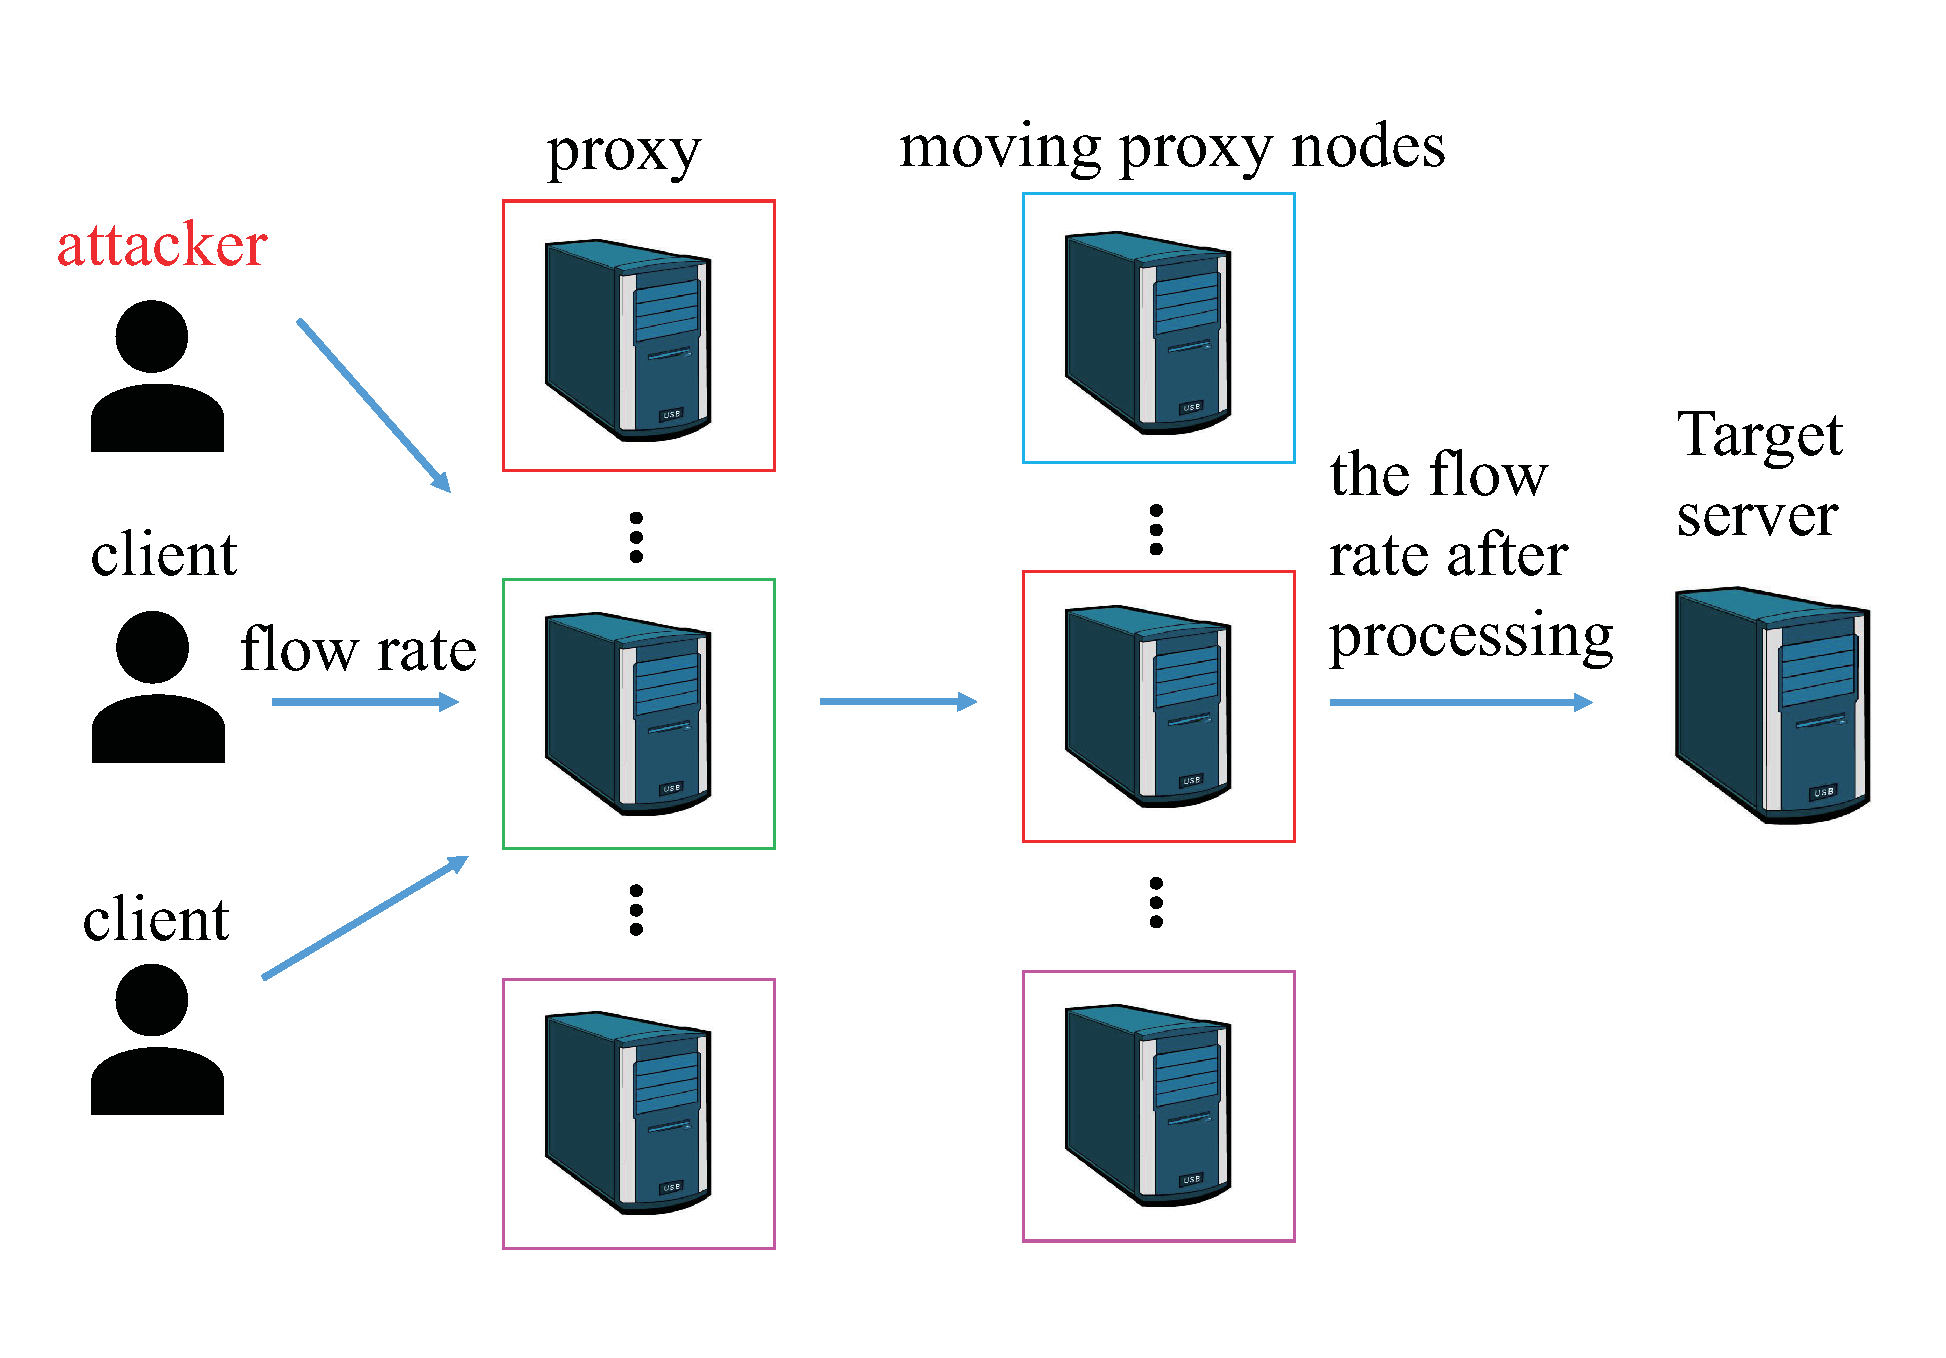
\includegraphics[width=1.0\linewidth,height=3.3in]{output/fig18.eps}
	\caption{DDOS defense method of secret moving proxy nodes.The
		proxy node is constantly moving its position, confusing the attacker
		so that it cannot find the real target server.}
	\label{fig18}
\end{figure}


Wang et al.~\cite{wang2014moving} propose a mobile target defense mechanism that specifically
addresses DDoS attacks targeting authenticated clients of Internet services.
This mechanism utilizes a set of dynamic and hidden proxies to relay traffic
between authenticated clients and servers. As shown in Fig.~\ref{fig18}, by continuously
replacing the attacked proxies with backup proxies and reallocating attacked
clients to new proxies, innocent clients are separated from malicious insiders
through a series of shuffling. In recent years, significant efforts have been
made to defend against lowrate DDoS attacks. Attackers easily launch complex
lowrate DDoS attacks by exploiting prominent features of cloud computing.
Therefore, research on various DDoS attacks and their corresponding defense
methods is crucial in protecting cloud infrastructure from devastating impacts
of DDoS attacks. Agrawal et al.~\cite{agrawal2019defense} conduct a comprehensive classification of
all possible variants of cloud DDoS attack solutions and provide detailed
insights into characterization, prevention, detection, and mitigation mechanisms.

In the future, these defense methods can be further
developed by constructing more secure and robust
encryption protocols and algorithms. Additionally, more effective
Identity verification technologies can be developed to
ensure the trustworthiness of communication parties.
Continual improvement and enhancement of transport layer
protocols, such as SSL/TLS, can provide stronger security
and defense capabilities, including the ability to resist
man-in-the-middle attacks, data tampering, and replay
attacks. The development of real-time threat detection
systems capable of detecting and responding to attacks
during the transmission process can also be explored.With
the advancement of quantum computing, traditional
encryption algorithms may be threatened. Therefore,
researching and developing quantum-safe communication
protocols and algorithms is also important to ensure
security during the transmission process and protect data
confidentiality in a quantum computing environment.

\subsection{Defense Against Model Aggregation Attack}
Defense methods against model aggregation attacks
include designing robust aggregation algorithms and using
differential privacy techniques to protect model parameters.

El Mhamdi et al.~\cite{guerraoui2018hidden} argue that mere convergence of
the Byzantine resilient rules is not enough. It is possible
that Byzantine workers' attacks can lead to convergence
to the worst suboptimal solution. To address this, they
propose a generic enhancement method called Bulyan.
This method significantly reduces the leeway for
Byzantine workers, constraining them within narrow boundaries.
For common batch sizes, Bulyan achieves performance
comparable to average speed.

Li et al.~\cite{li2014resolving},Hsu et al.~\cite{hsu2019measuring} and Jiang et al.~\cite{jiang2023secure}
work on issues about data heterogeneity and conflicts.
Li et al.~\cite{li2014resolving} model the problem using an optimization
framework where ground truth and source reliability are
defined as two sets of unknown variables. The objective
is to minimize the overall weighted differences between
the ground truth and multiple-source observations, with
each source weighted by its reliability. This framework
can incorporate different loss functions to identify
features of various data types and has developed efficient
computing methods that effectively identify the true
information among conflicting data sources. Hsu et al.~\cite{hsu2019measuring}
present a method for synthesizing datasets with
continuous identical ranges and provide performance
metrics for the federated averaging algorithm. Experimental
results demonstrate that performance deteriorates with
distribution differences. The proposed method suppresses
oscillations through the accumulation of gradient history,
and it has been shown that using momentum on top
of SGD for non-iid problems has achieved significant
success in accelerating network training. Jiang et al.~\cite{jiang2023secure}
introduce the combination of handling imbalanced data
and Byzantine attacks in the context of federated learning
for the first time. The concept of an intelligence pool is
proposed to separate the task of judging the shared local
model values from the aggregator, avoiding the limitations
of a single criterion through two-layer verification shown
in Fig.~\ref{fig19}.

Xie et al.~\cite{xie2018generalized},Portnoy et al.~\cite{portnoy2020towards} and Pillutla et
al.~\cite{pillutla2022robust} propose several rules or algorithms to make
the model aggregation work smoothly. Xie et al.~\cite{xie2018generalized}
introduce three robust aggregation rules for stochastic
gradient descent (SGD) with low computational costs.
These rules are the first to be theoretically and empirically
studied under the non-convex setting, based on median
aggregation. Portnoy et al.~\cite{portnoy2020towards} propose a novel method
called Byzantine Robust Client Weighting (BRCW) to
minimize the impact of malicious clients in federated
learning. BRCW assigns different weights to each client
based on their credibility and contribution to the overall
model accuracy. During training, the weights are
dynamically updated according to each client's performance
and behavior. Unlike previous work, this study considers
the sample size provided by clients as untrustworthy,
as it may come from malicious clients. BRCW exhibits
robustness against various forms of attacks, including
communication disruptions and data poisoning. Pillutla
et al.~\cite{pillutla2022robust} design a novel robust aggregation oracle based
on classical geometric medians and demonstrate its
robustness in federated learning with limited heterogeneity, even
when up to half of the devices are faulty. The proposed
RFA algorithm outperforms the standard FedAvg (14)
in high damage scenarios and nearly matches FedAvg's
performance in low damage scenarios, but with 1-3 times
higher communication costs.

\begin{figure}[h]
	\centering
	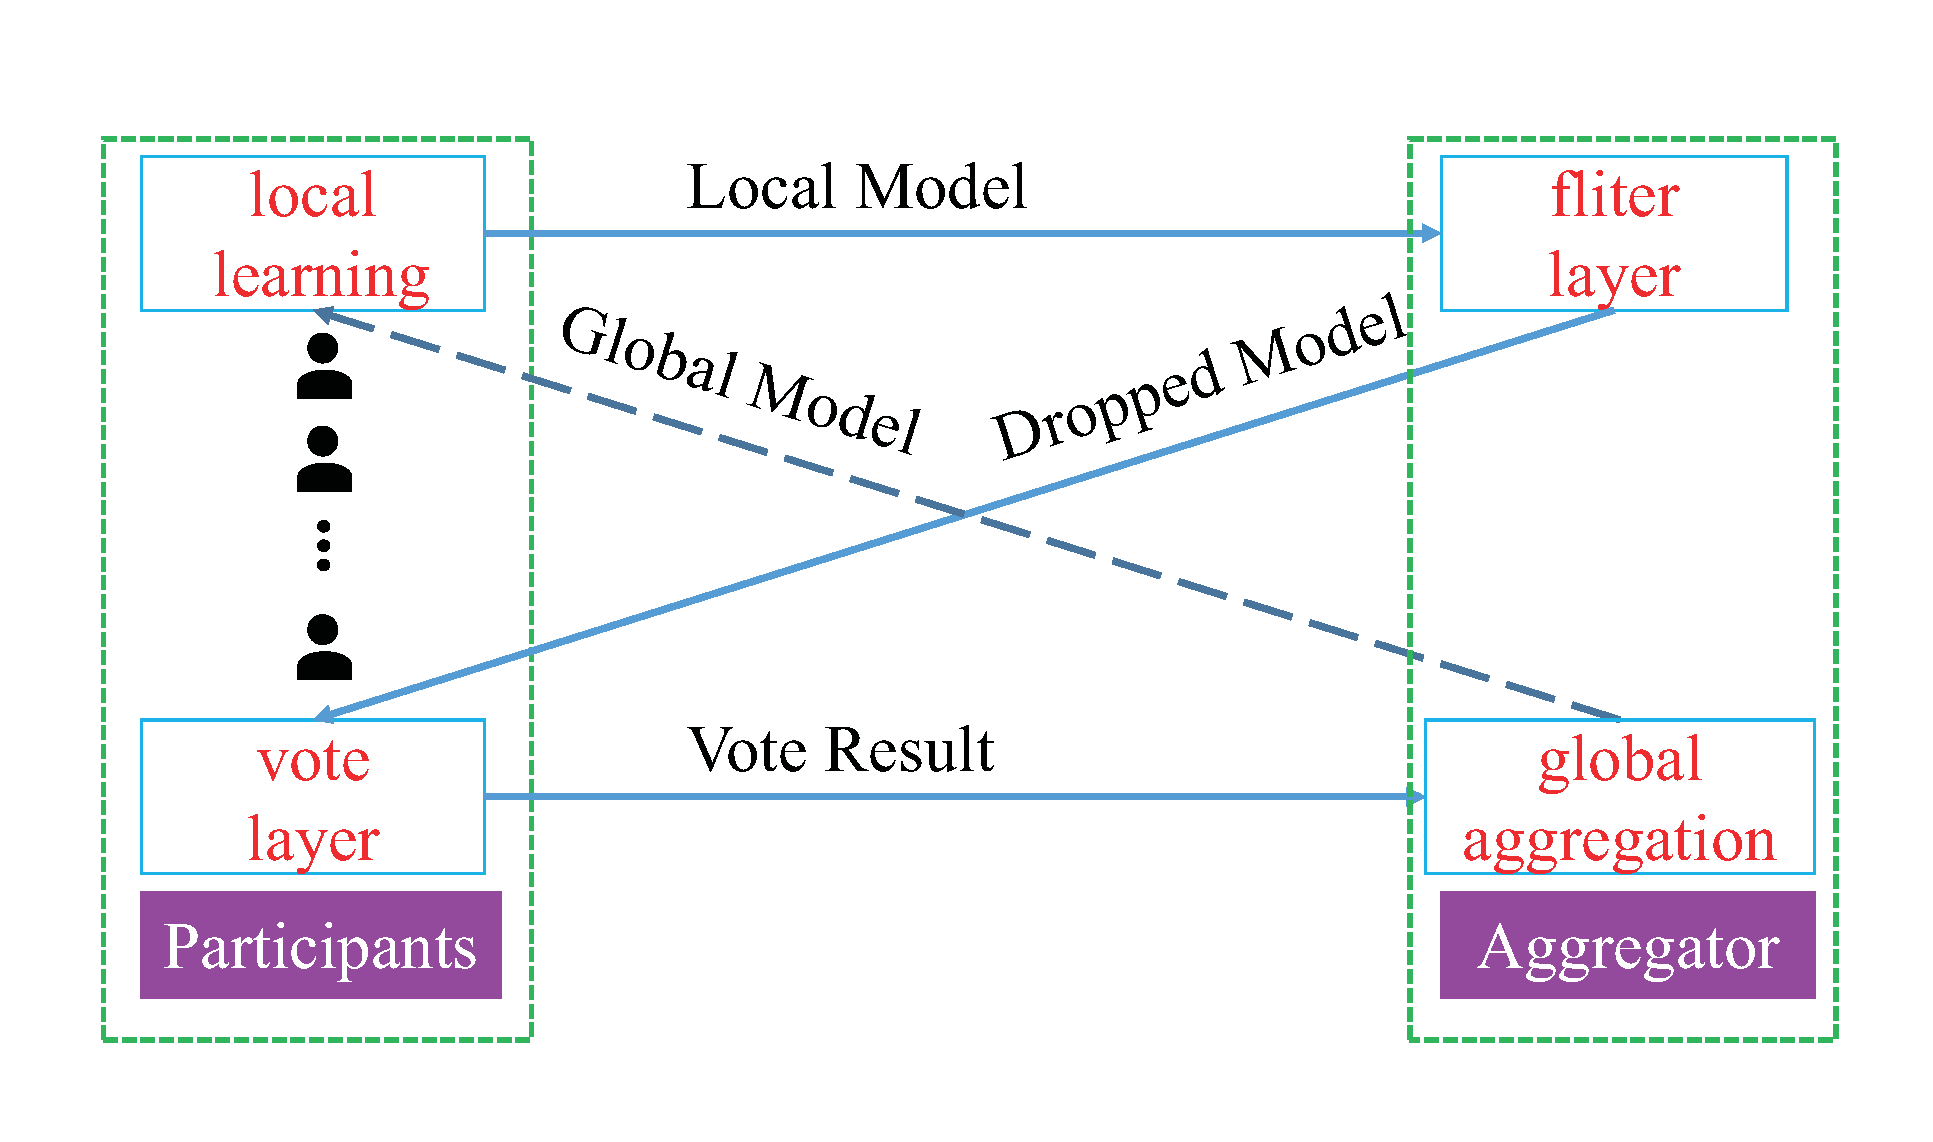
\includegraphics[width=1.0\linewidth,height=2.8in]{output/fig19.eps}
	\caption{The structure of two-layer aggregation method. Participants
		share the global model, and models discarded by the filter layer are
		not directly abandoned, but are voted by participants to participate
		in the final aggregation process.}
	\label{fig19}
\end{figure}


Future prospects for such defense methods will
focus on more stricter authentication and authorization
mechanisms, as well as parameter integrity protection.
Mechanisms such as Hash algorithms or digital signatures
can be adopted to safeguard the integrity of parameters,
preventing tampering during transmission and storage.
Detection of malicious parameter modifications and
corresponding response measures are also required.
By comprehensively applying these methods, the defense capability
against malicious parameter modification attacks can be
enhanced, ensuring the security and integrity of systems
and applications.


\section{Adversarial Attack}
Both adversarial attacks and backdoor attacks are techniques used to modify benign testing samples in order
to make models misbehave during the inference process. While adversarial perturbations are sample-agnostic in
universal adversarial attacks, these attacks can appear similar to backdoor attacks. Consequently, researchers
who are unfamiliar with backdoor attacks may question their significance, as these attacks require additional
controls on the training process to some extent. However, despite certain similarities, these attacks have essential
differences.

Firstly, adversarial attackers need to control the
inference process to a certain degree but not the training
process of models. They must query the model results
or even gradients multiple times to generate adversarial
perturbations by optimization, given a fixed targeted
model. On the other hand, backdoor attackers require
modifying certain training stages, such as data collection
and model training, without any additional requirements
in the inference process. Secondly, from the perspective
of attacked samples, backdoor attackers use known,
non-optimized perturbations, whereas adversarial attackers
require obtaining them through the optimization process
based on the model output. This optimization in
adversarial attacks requires multiple queries, making them unable
to be real-time in many cases. Finally, the mechanisms
of these attacks are fundamentally different. Adversarial
vulnerability results from the differences in behaviors of
models and humans, while backdoor attackers exploit the
excessive learning ability of deep neural networks (DNNs)
to establish a latent connection between trigger patterns
and target labels.

In federated learning, because the data is not shared
among participants, attackers can use this to generate
adversarial samples locally, then inject them into the data
sets of participants, and train the model with the data of
other participants during the training process.
So, how should attacks targeting federated learning be
designed? In centralized learning, FGSM~\cite{goodfellow2014explaining} is initially
used to generate adversarial examples. Let $\theta$ be the parameters of a model, $x$ the input to the model,
$eta$ the perturbation to original input and $||\eta||_\infty \le \epsilon$,
$y$ the targets associated with $x$ (for machine learning tasks that have targets)
and $J(\theta, x, y)$ be the cost used to train the neural network.
We can linearize the cost function around the current value of $\theta$,
obtaining an optimal max-norm constrained pertubation of:
\begin{equation}
	\eta = \epsilon sign(\nabla_x J(\theta,x,y))
\end{equation}

In federated learning, attackers can use FGSM locally
to generate adversarial samples and then inject them into
the datasets of some participants to affect the performance
of the entire model. PGD~\cite{madry2017towards} is a more powerful adversarial sample
generation method, which generates adversarial samples
by iteratively perturbing the input. Specifically, PGD
first randomly generates an initial disturbance $\delta_0$,
and then iteratively updates the disturbance $\delta_t$, to meet the constraint,
that is, $|\delta_t|_{\infty} \leq \epsilon_{\text{max}}$,
where $\epsilon_{\text{max}}$is the maximum value of the disturbance.
After each update, PGD also projects the disturbance
$\delta_t$ back into the constraint space to ensure that it meets the
constraint conditions.
Specifically, the update formula for PGD is as follows:
\begin{equation}
	x^{t+1} = \text{Clip}(x + \text{sign}(\nabla_x L(\theta,x',y)) \cdot \epsilon{\text{max}}, x - \epsilon_{\text{max}}, x + \epsilon_{\text{max}}),
\end{equation}
Where $\text{Clip}$ means to cut $x$ into the interval, and $\epsilon_ {\text{max}} $is the maximum value of the disturbance.
Unlike FGSM, PGD requires multiple iterations to generate adversarial examples,
so attackers need to use the local dataset and model parameters of each participant
to iteratively update the perturbation.

In federated learning, using PGD (Projected Gradient Descent) or FGSM
(Fast Gradient Sign Method) to generate adversarial examples and perform
adversarial attacks is a common method. However, compared to centralized
learning, there are some considerations and techniques that need to be
taken into account.

(1) Distribution Heterogeneity: In
federated learning, data is typically distributed across
various edge devices, making it slightly more difficult to
generate adversarial examples and perform attacks.
The differences from distribution heterogeneity can result in significant discrepancies between the aggregated server model and the client models,
which may lead to adversarial samples generated by the client models being ineffective in successfully attacking the newly aggregated server model.


(2)Network Latency and Bandwidth Limitations:
In federated learning, devices communicate through a
network, which may result in network latency or
bandwidth limitations. Therefore, when generating adversarial
examples and performing attacks, these factors need to
be taken into consideration. For example, it may be
necessary to optimize the size and generation speed of
adversarial examples to adapt to network limitations. And
in federated learning, the training steps of each participant
are asynchronous, which may lead to synchronization
issues. For example, attackers may not be able to perform
attacks on all participants' models because they may be
at different training steps or states.

(3)Update of Attack Strategies: Due to the dynamic
nature of federated learning, attackers need to constantly
update their attack strategies to adapt to changes in the
learning model and data distribution. This may require
designing more complex attack strategies and using more
efficient optimization algorithms.

(4)Attack Detection and Defense: In federated learning,
adversarial attacks may be easier to detect due to the
distribution and usage of data. Therefore, it is necessary
to design adversarial examples that are more difficult to
detect or use more complex attack strategies to avoid
detection.

Overall, using PGD or FGSM to generate adversarial
examples and perform adversarial attacks in federated
learning require considering the characteristics and limitations of federated learning, including the heterogeneity
of data distribution, network latency and bandwidth limitations,
update of attack strategies, and attack detection
and defense. This may require designing more complex
and efficient attack strategies and adversarial example
generation methods.

\section{Defenses against Adversarial Attack}
\label{Defenses against Adversarial Attack}
Various adversarial examples have been great threats to
deep learning models. Naturally, many defense methods
are proposed to enhance the robustness of deep learning
models. As adversarial samples share similarities with the
previously discussed backdoor samples, defense methods
involving sample filtering can be employed.
The most common idea is to filter out adversarial samples from test data using a trained binary classifier~\cite{wang2024defense, wang2024detecting,zhang2023detecting}.
However, these methods develop specialized detectors for specific attacks or classifiers, 
which largely neglects the modeling of data distribution, resulting in their limited effectiveness against unknown attacks.
Moreover, according to the learning paradigm of federated learning, the server model cannot access the data from the client devices, which significantly limits the application of such defense methods in federated learning.

In this section, we focus on the defense method of adversarial
training. Adversarial training is a defense method against
adversarial attacks. Its basic idea is to incorporate
adversarial examples into the training process, enabling the
model to better withstand unknown adversarial attacks.
Specifically, adversarial training combines the original
training dataset with adversarial samples generated to
target the model, and retrain the model accordingly. This
way, the model encounters adversarial examples
continuously during the learning process, thereby enhancing
its robustness and generalization capability.

As shown in Fig.~\ref{fig20}, since adversarial training was first applied to
federated learning in 2020, there are problems in four
aspects. From these four aspects, we describe the current
state of development of federated adversarial training.
FAT (Federated Adversarial Training) is a method
proposed in~\cite{zizzo2020fat} that combines federated learning and
adversarial training to reduce evasion threats during
inference while preserving data privacy during training.
In the FAT protocol, each device trains a local model and
generates adversarial samples, which are mixed with the
original data for training. The models are then uploaded
to the server for aggregation. This helps to improve the
robustness of the model against adversarial attacks. The
authors note that the protocol does not work out of
the box and requires careful tuning of the optimization
parameters to achieve good results. Additionally, the
authors acknowledge that the experiments were conducted
on idealized federated settings and that further research
is needed to evaluate the effectiveness of FAT in more
realistic scenarios.

\begin{figure*}[h]
	\centering
	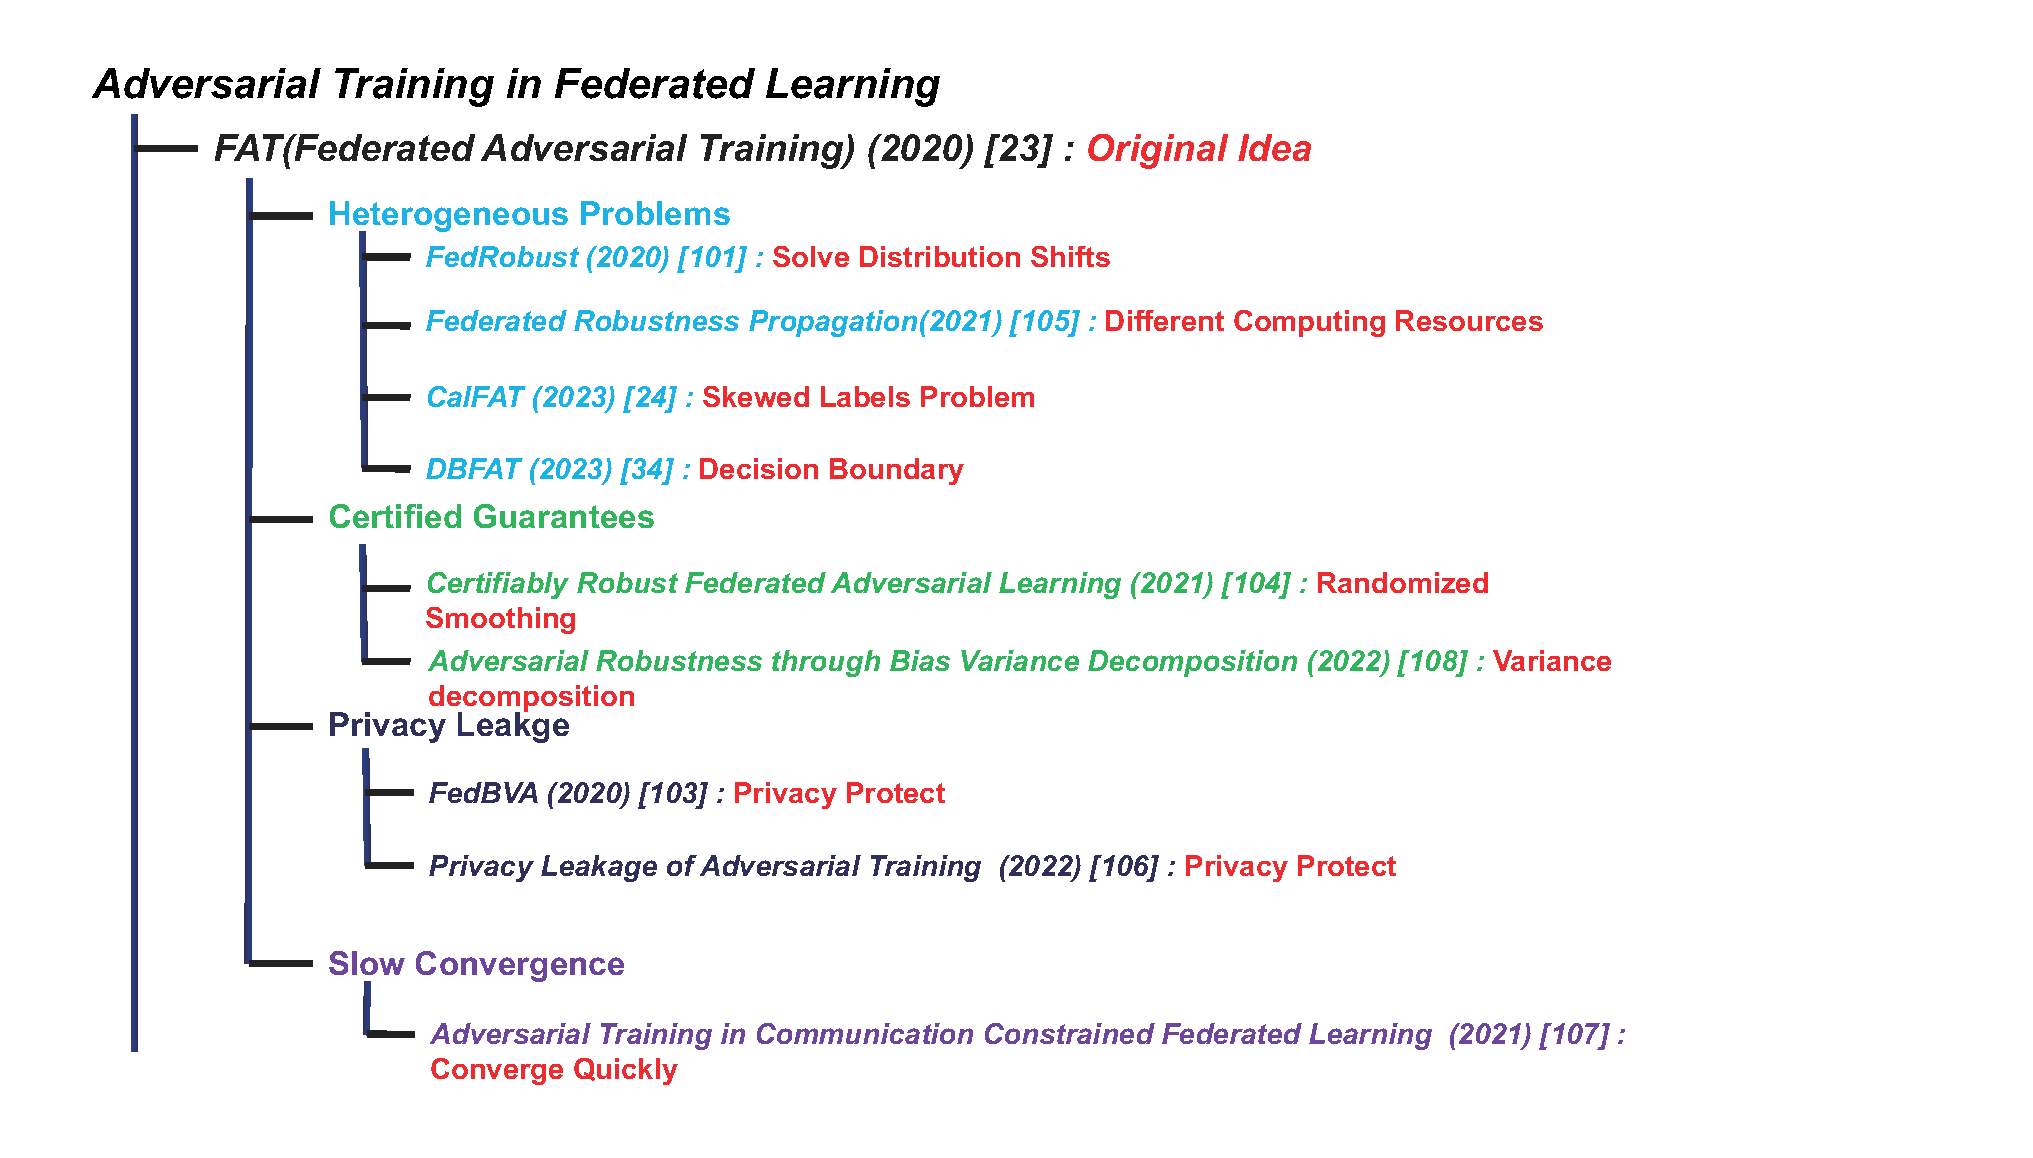
\includegraphics[width=1.0\linewidth,height=3.5in]{output/fig20.eps}
	\caption{The development of federated adversarial training.}
	\label{fig20}
\end{figure*}


So, there are also several challenges with
implementing adversarial training in federated learning, such as
heterogeneous clients caused by distribution, certified
guarantees, privacy leakage, and slow convergence rate.

\subsection{Heterogeneous Clients Caused by Distribution}
The major challenge in federated learning is the
heterogeneity of clients. This means that the distribution of
training data may vary among different clients, and the
computational resources available to each client may also
differ. The paper~\cite{reisizadeh2020robust} proposes a novel method called
FedRobust to address the problem of distribution shifts
in federated learning. FedRobust is a gradient descent
ascent (GDA) algorithm that solves the minimax robust
optimization problem and can be efficiently implemented
in a federated setting. This paper shows that FedRobust,
which alternates between the perturbation and parameter
model variables, will converge to a stationary point in the
minimax objective that satisfies the Polyak-Łojasiewicz
(PL)~\cite{polyak1963gradient} condition. This optimization method can be
used to address the issue of distribution shifts in federated
learning, which can significantly impact the performance
of the trained model.

\begin{figure}[h]
	\centering
	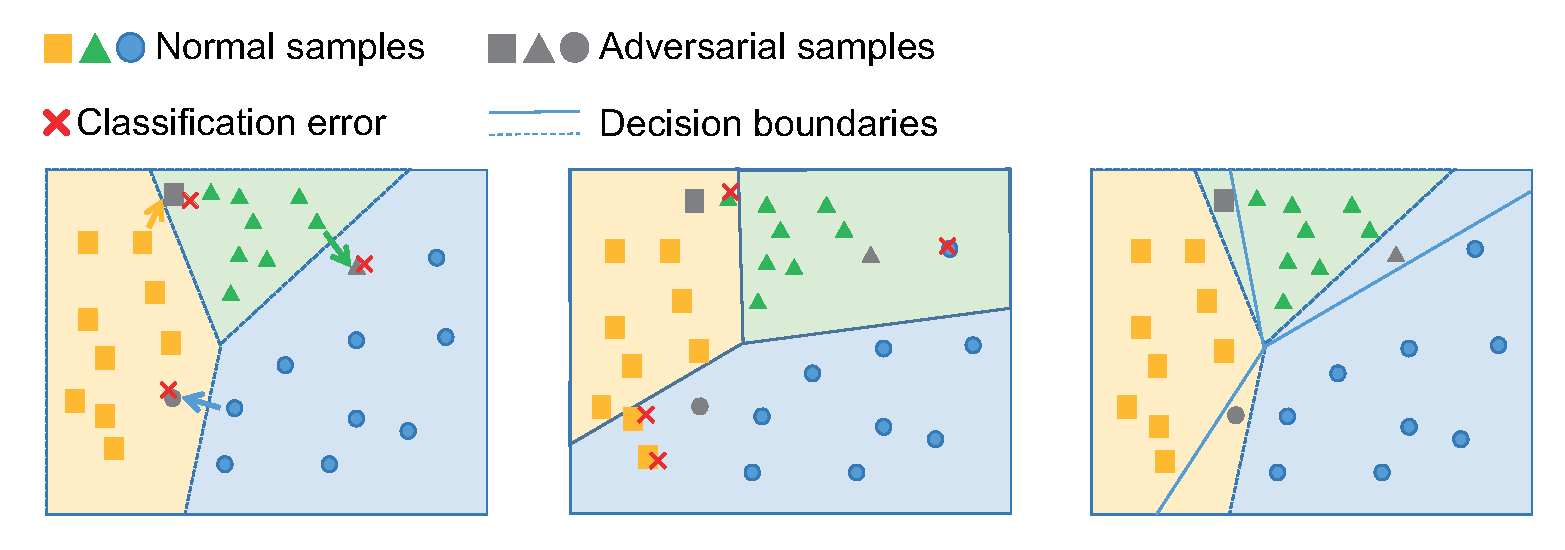
\includegraphics[width=1.0\linewidth,height=1.8in]{output/fig21.eps}
	\caption{Decision boundary of DBFAT-trainedmodel.}
	\label{fig21}
\end{figure}


Zhang et al.~\cite{zhang2023delving} find that the accuracy of the federated
learning model with adversarial training decreases on
clean data, especially when the data of different clients
are non-independent and identically distributed, so they
propose an algorithm based on decision boundary as
shown in Fig.~\ref{fig21}, which uses local reweighting and global
regularization to improve the accuracy and robustness in
federated adversarial training. Chen et al.~\cite{chen2022calfat} study the
skewed labels problem in federated learning and proposes
a CalFAT framework to calculate the logits of each class.
By using this framework, the models between different
clients eventually converge, enhancing the robustness and
accuracy of the global model.
Hong et al.~\cite{hong2021federated} have studied the problems caused
by clients with different computing resources. During
federated learning, some clients can support adversarial
training, but some clients with lack of computing resources
can not support it. This paper studies how to spread
resistance robustness from resource-rich users who can
support confrontation training to those users with poor
resources. This paper shows that an effective robust
propagation algorithm is proposed by using BN layer
technology correctly.

\subsection{Certified Guarantees}
Certified guarantees are needed in adversarial training
to ensure reliable protection and security against unknown
attacks in adversarial environments. Certified guarantees
refer to rigorous proofs and assurances of model
performance. They provide protection bounds against specific
types of attacks, indicating that the model can maintain
a certain level of performance regardless of how carefully
the attacker designs the attack, such as high accuracy or
robustness.

By using certified guarantees, adversarial training can
provide a degree of predictability and security. This means
that in practical deployment, there is higher confidence in
the model's performance and trustworthiness, rather than
relying solely on trial-and-error evaluation and protection.
It offers a more reliable and definitive defense mechanism
for models to handle unknown or complex attacks.
Chen et al.~\cite{chen2021certifiably} propose incorporating randomized
smoothing techniques into federated adversarial training
to enable data-private distributed learning with
certifiable robustness to test-time adversarial perturbations.
The experiments conducted in the paper show that this
approach can deliver models as robust as those trained
by centralized training, and can enable provably-robust
classifiers to 2-bounded adversarial perturbations in a
distributed setup.

From the perspective of variance-bias decomposition,
Zhou et al.~\cite{zhou2022adversarial} decompose the loss function into a
combination of bias and variance, generate adversarial
samples on the server and return them to each client for
adversarial training. Then, they used any model
aggregation algorithm to improve the global model's adversarial robustness.

\subsection{Privacy Leakage}
As mentioned earlier, privacy protection is crucial in
federated learning. In~\cite{zhang2022privacy}, it is proved that the model of
confrontation training is more prone to privacy disclosure
than the model of normal training. Zhou et al.~\cite{zhou2020adversarially}
argue that conventional federated learning frameworks are
vulnerable to strong adversarial attacks, even if adversarial
training using locally generated adversarial examples is
performed on each client. To address this problem, the
paper proposes a new framework called FedBVA (Federated
Learning with Bias-Variance Analysis) that provides a tiny
amount of bias-variance perturbed data from the central
server to the clients through asymmetrical communication.
This approach dramatically improves the robustness of the
training model under various settings, without violating
the clients' privacy.

\subsection{Slow Convergence Rate}

As described in~\cite{zhang2023delving}, conducting adversarial training
in federated learning is a challenging task because the
convergence speed of adversarial training is very slow.
In~\cite{shah2021adversarial}, a method is proposed to solve this problem.
Assuming the local iteration number of federated learning
is E, this article believes that a larger E will increase the
drift between models and affect the adversarial robustness,
but will converge quickly. A smaller E will increase
the adversarial robustness but decrease the convergence
efficiency. Therefore, this article proposes a dynamic
mechanism for adjusting E, and uses FedCurv instead of
FedAvg as the global aggregation algorithm, and proposes
a new algorithm called FedDynAT to simultaneously
improve the convergence speed and adversarial robustness.
As shown in Tab.\ref{Comparison of FAT}, we list some of the methods
mentioned above for comparison. It can be seen from the
table that the adversarial robustness in federated learning
is still weak (less than 40\%). Therefore, the study of
adversarial training in federated learning is still a very
urgent matter.


\begin{table}[t]
    \caption{\textbf{Comparison of Federated Adversarial Training}}
    \label{Comparison of FAT}
    \centering
    \begin{tabular}{|c|c|c|c|} % 有七列,使用 "c" 表示居中对齐,没有竖线
    \toprule % 第一道横线
    \textbf{Methods}  & \textbf{Accuracy} & \textbf{PGD-Robustness} & \textbf{AA-Robustness}\\ 
    \midrule
     MixFAT& $53.75\%$ &   $29.61\%$ &   $21.59\%$ \\
     \midrule
     FedRBN& $47.80\%$ &  $26.87\%$ & $20.46\%$ \\
     \midrule
     CalFAT& $64.69\%$ & $32.59\%$  & $22.83\%$ \\
     \midrule
     DBFAT& $52.16\%$ &  $27.80\%$ & $-$ \\
     \midrule
     FedBVA& $83.8\%$ &  $21\%$ & $-$ \\
     \midrule
     FedPGD& $49.57\%$ &  $28.48\%$ &  $21.34\%$ \\
     \midrule
     FedAvg& $80.5\%$ &  $9.9\%$ & $-$ \\
    \toprule
    % 继续插入更多数据行
    \end{tabular}
    \end{table}  


    \section{Advanced Research and Problems}
    \label{Advanced Research and Problems}
    \subsection{Stealthiness}
    
    A good attack method should not be easily detected by
    the defense system. Backdoor attackers need to effectively
    hide backdoors to make them difficult to detect. In
    Byzantine attacks, how do Byzantine attackers launch
    attacks while evading detection is also to be solved.
    Adversarial attacks need to generate adversarial samples
    without being detected. The attack methods developed
    above enhance their stealthiness by exploiting long-tail
    distribution, federated learning distribution, and dynamic
    generation techniques. Long tail distributed attacks and
    distributed attacks will eventually be discovered by the
    larger and larger model capacity, so how to develop a
    hidden attack method that can effectively face the large
    capacity model is a major problem in the current attack
    method research.   
    
    \subsection{Trade-Off}
    There are many Trade-off issues in federated learning.
    In federated learning, client data is distributed among
    multiple participants. The protection of privacy is an
    important reason why federated learning is so popular.
    So it is an important challenge to ensure data privacy
    while implementing defenses. Effective defense
    mechanisms, such as fault-tolerant algorithms and majority
    voting, are needed to counter Byzantine attacks. However,
    these mechanisms need to strike a balance with factors
    like privacy preservation and computational efficiency.
    Adversarial training can enhance model robustness but
    may compromise generalization capability. Balancing the
    trade-off between adversarial robustness and
    generalization is a problem that requires exploration and resolution.
    Recently, some works have studied the latent connection
    between adversarial attacks and backdoor attacks. For
    example, Weng et al.~\cite{weng2020trade} empirically demonstrated that
    defending against adversarial attacks via adversarial
    training may increase the risks of backdoor attacks. Solving
    these various Trade-off problems is also the focus of future
    research in federated learning.
    
    \subsection{Convergence}
    In defense methods, in order to improve the robustness
    of the model, existing methods often improve the training
    process of the model, such as distillation or adversarial
    training. These methods do play a good defense effect, but
    also bring the model convergence problems. The distributive
    nature of federated learning further aggravates the
    problem of difficult convergence, because the distributive
    nature may cause problems such as heterogeneous data
    and unbalanced computing resources. In the methods
    mentioned in this paper, some articles have improved these
    problems in defense methods, such as using smoothing
    to produce equivalent results, or using reweighting to
    improve decision boundaries to solve the impact of data
    heterogeneity. But in general, how to make the model
    converge quickly is still a problem that needs to be studied
    in the future.
    \section{Conclusion}
    In this survey, we systematically introduce state of the art 
    threats in federated learning systems, which mainly
    include byzantine attacks, backdoor attacks and adversarial
    attacks. And we also detailed describe corresponding
    defensive policies. We also introduce the advantages and
    disadvantages of these methods and how they work, and
    sort out the relationship between them. Additionally, we
    discuss a number of open problems of current defense
    methods, hoping them could help researchers identify and
    solve issues more quickly in the area of robust federated
    learning.




%%===========================================================================================%%
%% If you are submitting to one of the Nature Portfolio journals, using the eJP submission   %%
%% system, please include the references within the manuscript file itself. You may do this  %%
%% by copying the reference list from your .bbl file, paste it into the main manuscript .tex %%
%% file, and delete the associated \verb+\bibliography+ commands.                            %%
%%===========================================================================================%%

\bibliography{sn-bibliography}% common bib file
%% if required, the content of .bbl file can be included here once bbl is generated
%%\input sn-article.bbl


\end{document}
